%!TEX program=xelatex

% 碰到Windows版本提示Fandol字体,可以在命令行中以管理员权限执行:tlmgr update -self -all
\documentclass[final]{cvpr}

\usepackage[UTF8]{ctex}

%\usepackage{cvpr}
\usepackage{times}
\usepackage{epsfig}
\usepackage{graphicx}
\usepackage{amsmath}
\usepackage{amssymb}
\usepackage{subfigure}
\usepackage{overpic}
\usepackage{booktabs} % 推荐添加:用于制作更专业的三线表

\usepackage{enumitem}
\setenumerate[1]{itemsep=0pt,partopsep=0pt,parsep=\parskip,topsep=5pt}
\setitemize[1]{itemsep=0pt,partopsep=0pt,parsep=\parskip,topsep=5pt}
\setdescription{itemsep=0pt,partopsep=0pt,parsep=\parskip,topsep=5pt}

\usepackage[pagebackref=true,breaklinks=true,colorlinks,bookmarks=false]{hyperref}

%\cvprfinalcopy % *** Uncomment this line for the final submission

\def\cvprPaperID{****} % *** 在此处输入论文ID
\def\confYear{CVPR 202X}
\def\httilde{\mbox{\tt\raisebox{-.5ex}{\symbol{126}}}}

% 自定义命令
\newcommand{\mypara}[1]{\paragraph{#1.}}
\renewcommand{\figref}[1]{图\ref{#1}}
\renewcommand{\tabref}[1]{表\ref{#1}}
\renewcommand{\equref}[1]{式\ref{#1}}
\renewcommand{\secref}[1]{第\ref{#1}节}

% 页面设置
\setcounter{page}{1}

\begin{document}
\setcounter{tocdepth}{2}

\def\abstract{\centerline{\large\bf 摘要} \vspace*{12pt} \it}

%%%%%%%%% 标题部分
\title{SDXL 1.0 文生图 与 Flux.1 Kontext Dev 图像编辑探索性实验}

\author{李衡\\学号:23354088\\课程名称:计算机视觉\\课题选择:Task1$\boxed{\checkmark}$ Task2$\boxed{\checkmark}$ \\
     中山大学 \quad 智能工程学院
}

\maketitle

%%%%%%%%% 摘要
\begin{abstract}
随着生成式人工智能技术的演进,扩散模型已从基础的图像生成迈向了高精度的可控编辑阶段。本报告基于 ComfyUI 实验平台,系统性地评估了 SDXL 与 FLUX.1 两大主流开源模型在不同任务场景下的性能表现与参数敏感性。

针对 SDXL 的文生图(Text-to-Image)任务,本文采用控制变量法深入分析了采样步数、提示词引导系数(CFG Scale)及分辨率对生成质量的影响。实验结果表明,CFG Scale 在 3.0 左右实现了指令遵循与画面自然度的最佳平衡,而分辨率与采样步数的设定需严格契合模型的训练分布与收敛特性以避免结构崩坏。

针对 FLUX.1 Kontext Dev 的图像编辑(Image-to-Image)任务,本文聚焦于多模态输入的语义理解与重构能力。通过对“鸭公主”与“兔公主”样本的实证分析,对比了不同采样算法与调度策略的效能。研究发现,Euler 采样器配合 Simple 调度器构成了该流匹配模型的最佳推理组合,有效克服了 DDPM 的噪点残留与 Karras 策略的模糊伪影。同时,实验验证了 Flux 引导系数在风格迁移与细节增强上的调控作用,以及模型在复杂场景切换中维持角色特征一致性的卓越能力。

\textbf{关键词:} 扩散模型;SDXL;FLUX.1;图像编辑;参数敏感性分析;ComfyUI
\end{abstract}
% \newpage % 换页

% ==========================================
% 3. 生成目录 (核心命令)
% ==========================================
\tableofcontents
\newpage % 目录通常单独占一页,所以这里强制换页
%%%%%%%%% 正文部分
\section{部分结果展示}
\begin{figure}[h]
    \centering
    \includegraphics[width=0.5\textwidth]{example.png}
    \caption{UI部署}
    \label{fig:example}
\end{figure}

\begin{figure}[h] % [t] 表示强制置顶,figure* 表示跨双栏(如果是双栏排版)
    \centering
    % 请确保图片文件名与脚本生成的一致
    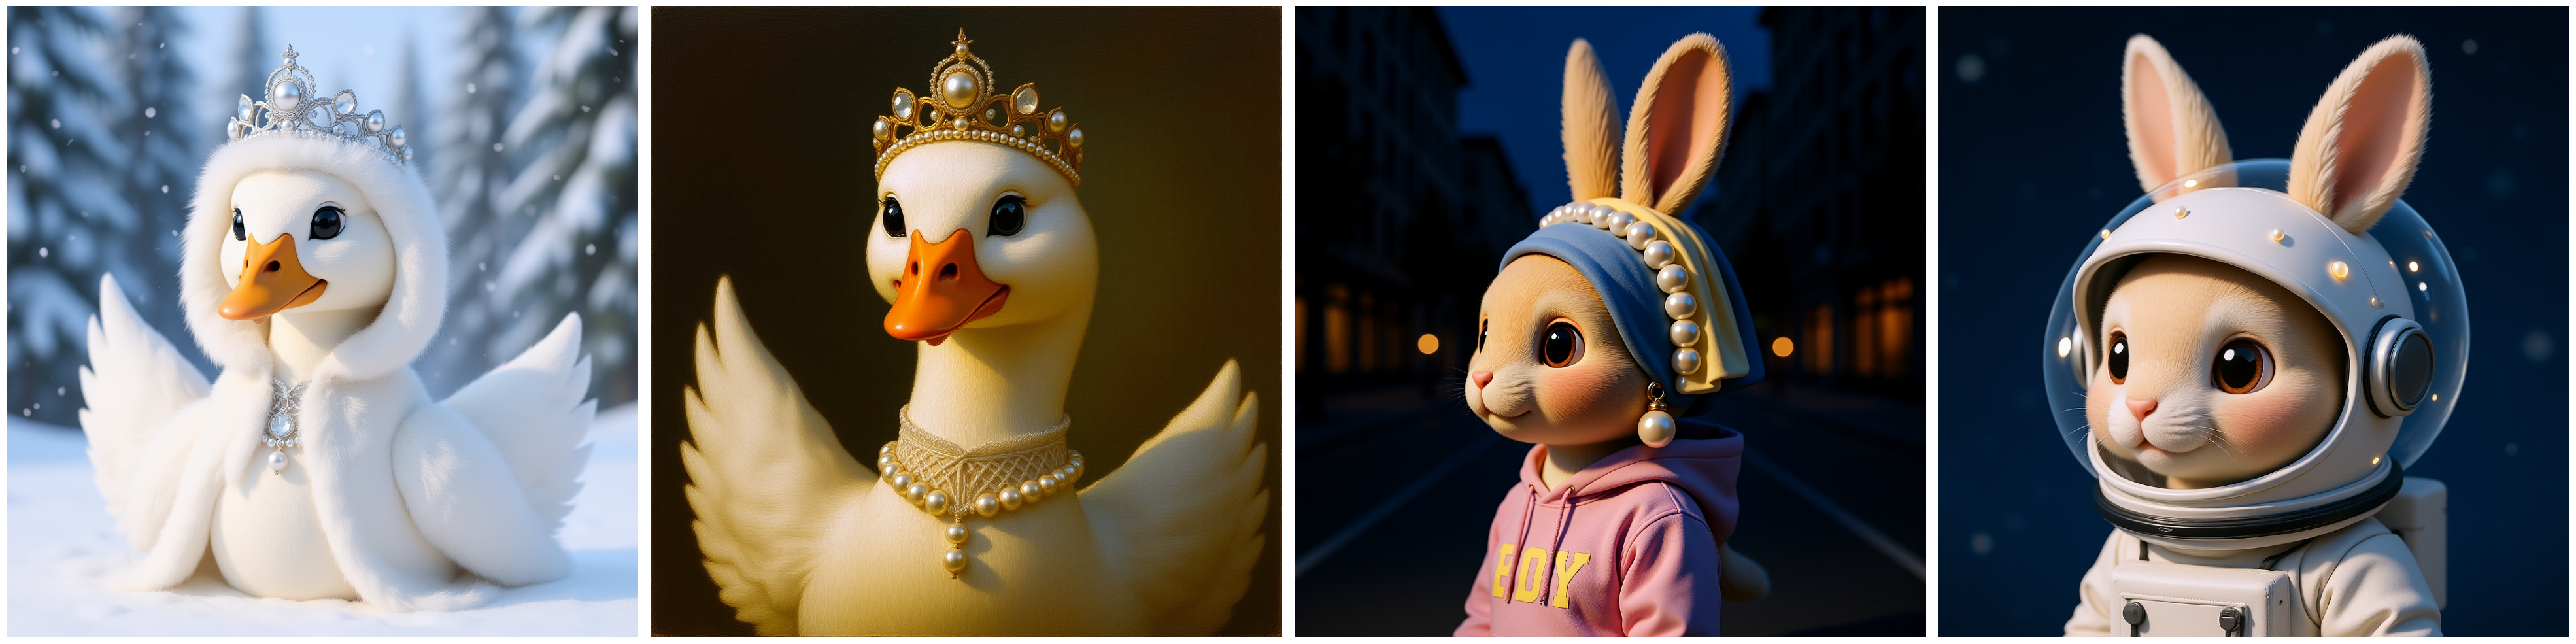
\includegraphics[width=0.5\textwidth]{showcase_merged.png}
    
    \caption{\textbf{基于 FLUX.1 模型参数调优后的最佳生成效果展示。} 
    通过联合优化 Flux 引导系数 (Guidance)、采样器 (Sampler) 及调度策略 (Scheduler),模型在多样化的生成任务中均展现出卓越的性能。}
    \label{fig:teaser_showcase}
\end{figure}

\section{引言}\label{sec:Introduction}

随着人工智能生成内容(AIGC)技术的飞速发展,基于扩散模型(Diffusion Models)的图像生成与编辑技术已成为计算机视觉领域的核心研究方向。从高质量的文本生成图像(Text-to-Image)到精细化的图像编辑(Image-to-Image),这些技术正在重塑数字内容创作的工作流。本实验报告旨在通过 ComfyUI 平台,系统性地探索当前主流开源模型的性能表现与应用边界,主要包含以下两个维度的研究任务。

第一部分聚焦于\textbf{文生图(Text-to-Image)}技术的参数行为分析。文本生成图像的核心在于将抽象的语义描述转化为具体的像素表达,而生成结果的质量与连贯性深受模型推理超参数的影响。在本任务中,我们将采用 \textbf{SDXL} \cite{sdxl}模型配合 ComfyUI 官方示例工作流,通过控制变量法进行实验。我们将重点探究\textbf{采样步数(Sampling Steps)}、\textbf{提示词引导系数(CFG Scale)}以及\textbf{图像分辨率}这三个关键参数对生成结果的影响。通过在固定随机种子和提示词的前提下对比不同参数组合的输出,旨在深入理解扩散模型在去噪过程中的行为逻辑,以及各参数如何权衡生成效率与图像质量。

第二部分探讨\textbf{图像到图像编辑(Image-to-Image Editing)}的多维应用。相较于从零开始的生成,对现有图像进行可控的编辑在实际应用中更具挑战性。本任务基于 \textbf{FLUX.1 Kontext Dev} ~\cite{flux}模型及其官方工作流,对真实图片进行多样化的编辑测试。实验内容涵盖四个方面:\textbf{基础属性修改}(如颜色、时间与天气的变换)、\textbf{艺术风格迁移}(如油画与素描风格化)、\textbf{保持主体一致性的场景替换}以及\textbf{简单的文本内容编辑}。通过调节相关参数,我们将验证该模型在保持原图特征基础上的语义理解与重绘能力。

综上所述,本文通过一系列定性与定量的实验,旨在展示并分析 SDXL 与 FLUX.1 在当前生成式 AI 任务中的实际控制机理与应用潜力。

\section{方法与实现原理}\label{sec:Methodology}

本节将概述实验所涉及的核心模型架构与技术背景,重点剖析用于文生图任务的 SDXL 模型底层的扩散机制,以及用于图像编辑任务的 FLUX.1 模型中的编码器与 Transformer 架构。

\subsection{基于潜在扩散模型的文本生成图像 (SDXL)}

Stable Diffusion XL (SDXL) 是潜在扩散模型(Latent Diffusion Models, LDMs)的集大成者。为了在高分辨率下实现高效且高质量的生成,SDXL 在模型架构上进行了多维度的创新。

\subsubsection{潜在空间与扩散机制}
与直接在像素空间操作的传统扩散模型不同,SDXL 利用\textbf{变分自编码器 (VAE~\cite{vae})} 将图像从像素空间压缩至低维的潜在空间(Latent Space)。
\begin{itemize}
    \item \textbf{前向扩散过程:} 在训练阶段,模型逐步向潜在变量添加高斯噪声,直至其变为纯随机噪声。
    \item \textbf{反向去噪过程:} 生成过程则是这一过程的逆操作。SDXL 使用一个大规模的 U-Net~\cite{unet} 网络来预测并去除每一步的噪声。该 U-Net 的参数量约为 SD 1.5 的三倍,并引入了 Transformer 模块(Cross-Attention)将文本信息注入去噪过程。
\end{itemize}

\subsubsection{双文本编码器策略 (Dual Text Encoders)}
为了提升语义理解能力,SDXL 摒弃了单一文本编码器方案,转而采用\textbf{双编码器策略}。它同时加载了 OpenCLIP ViT-bigG/14 和 CLIP ViT-L/14~\cite{clip, vit}。前者侧重于捕捉细腻的语义描述,后者则擅长通用的图文对齐。两者的输出特征被拼接后送入 U-Net,使得 SDXL 既能理解简短的 Prompt,也能处理复杂的自然语言描述。

\subsubsection{专家混合流水线 (Ensemble of Experts)}
如实验设置所述,SDXL 采用了一种“基础模型+精炼模型”的流水线架构:
\begin{enumerate}
    \item \textbf{基础模型 (Base Model):} 负责生成图像的潜在变量(Latents),构建整体的构图与语义框架。
    \item \textbf{精炼模型 (Refiner Model):} 这是一个专门针对低噪声水平训练的独立模型。它接收基础模型生成的含噪潜变量,进行最终的高频细节去噪。这种分工协作确保了图像既有合理的结构,又具备逼真的纹理细节。
\end{enumerate}

\subsection{基于多模态流匹配的图像编辑 (FLUX.1 Kontext Dev)}

FLUX.1 代表了图像生成领域的最新范式转变。不同于 SDXL 的 U-Net 架构,FLUX.1 基于\textbf{整流流匹配 (Rectified Flow Matching)} 理论,并采用全 Transformer 架构(DiT),拥有 120 亿参数。

\subsubsection{混合文本编码与多模态理解}
FLUX.1 的强大理解能力源于其复杂的条件编码机制,特别是 \textbf{CLIP} 与 \textbf{T5} 的结合:
\begin{itemize}
    \item \textbf{CLIP (Contrastive Language-Image Pre-training):} FLUX 使用 CLIP 编码器将文本提示映射为与视觉特征对齐的向量。这确保了生成的图像在视觉上与文本描述高度契合。
    \item \textbf{T5 (Text-to-Text Transfer Transformer):} 为了处理复杂的指令(如 Task 2 中的文字编辑和逻辑推理),FLUX 引入了 T5-XXL 模型。T5 提供了强大的语言推理能力,使得模型能够理解“将A替换为B并保持风格”这类复杂的句法结构。
\end{itemize}

\subsubsection{变分自编码器 (VAE) 与压缩}
FLUX.1 配备了一个经过高度优化的 VAE。该 VAE 负责将高分辨率的 RGB 图像(如 $1024 \times 1024$)编码为紧凑的潜在表示(Latents)。在图像编辑任务中,VAE 的解码器(Decoder)起着至关重要的作用,它负责将经过 Transformer 处理后的潜在特征无损地还原为像素图像,确保了编辑后的图像在细节纹理上(如皮肤毛孔、材质光泽)依然保持照片级的真实感。

\subsubsection{Kontext Dev 的核心编辑能力}
本报告使用的 FLUX.1 Kontext [Dev] 版本是一个开源的扩散 Transformer 模型。该模型利用其 DiT 架构中的自注意力机制(Self-Attention),实现了对图像全局上下文的深度感知。其核心能力包括:
\begin{itemize}
    \item \textbf{角色一致性(Character Consistency):} 借助 Transformer 的长程依赖捕捉能力,模型能在多个场景中锁定并保留参考角色的独特特征。
    \item \textbf{精准编辑(Editing):} 通过理解文本指令与图像内容的对应关系,实现局部修改而不破坏整体结构。
    \item \textbf{风格参考(Style Reference):} 将参考图的风格特征注入生成的流场中,实现风格迁移。
    \item \textbf{交互速度(Interactive Speed):} 得益于流匹配算法的高效性,模型能在较少的步数内收敛,提供低延迟的交互体验。
\end{itemize}

\section{实验环境}

本实验的所有图像生成与编辑任务均在服务器高性能计算工作站上完成,以确保推理过程的稳定性与效率。硬件配置方面,核心计算设备采用了 \textbf{NVIDIA GeForce RTX 3090} 显卡(24GB VRAM),并配置了 \textbf{CUDA 11.7} 计算架构以提供底层的并行加速支持。

在实验模型方面,针对 Task 1 的文生图(Text-to-Image)任务,我们选用了 \textbf{sd\_xl\_turbo\_1.0\_fp16} 模型。该模型基于 SDXL 架构并进行了半精度(FP16)优化,能够在保证生成质量的前提下显著降低显存占用并提升推理速度。针对 Task 2 的图像编辑(Image-to-Image Editing)任务,我们加载了 \textbf{FLUX.1 Kontext Dev} 模型,利用其先进的 Transformer 架构与多模态理解能力,实现对图像的精准控制与编辑。
\section{实验结果及分析}
\subsection{SDXL文生图实验}\label{sec:Method}

本章聚焦于文本生成图像(Text-to-Image)任务,利用 ComfyUI 搭建的 SDXL 官方示例工作流开展实验。为了深入理解扩散模型的生成机理及各超参数的调节作用,我们采用了严格的控制变量法。实验过程中,我们固定了输入的提示词(Prompt)与随机种子(Seed),确保实验结果具有可比性,随后依次调整\textbf{采样步数(Sampling Steps)}、\textbf{提示词引导系数(CFG Scale)}以及\textbf{图像分辨率(Resolution)}这三个核心参数。通过对比不同参数配置下的生成图像,本节将详细阐述这些关键变量如何在图像清晰度、指令遵循性以及物理结构合理性等方面影响生成质量。

\subsubsection{采样步数对生成质量的影响分析}

采样步数(Sampling Steps)决定了扩散模型在去噪过程中迭代的次数。在本实验中,我们控制 CFG Scale 为 1.7,分辨率为 $512 \times 512$,将采样步数分别设置为 1、4、7 和 10,以观察图像生成质量的演变过程。实验结果如图 \ref{fig:steps_comparison} 所示。

\begin{figure}[h]
    \centering
    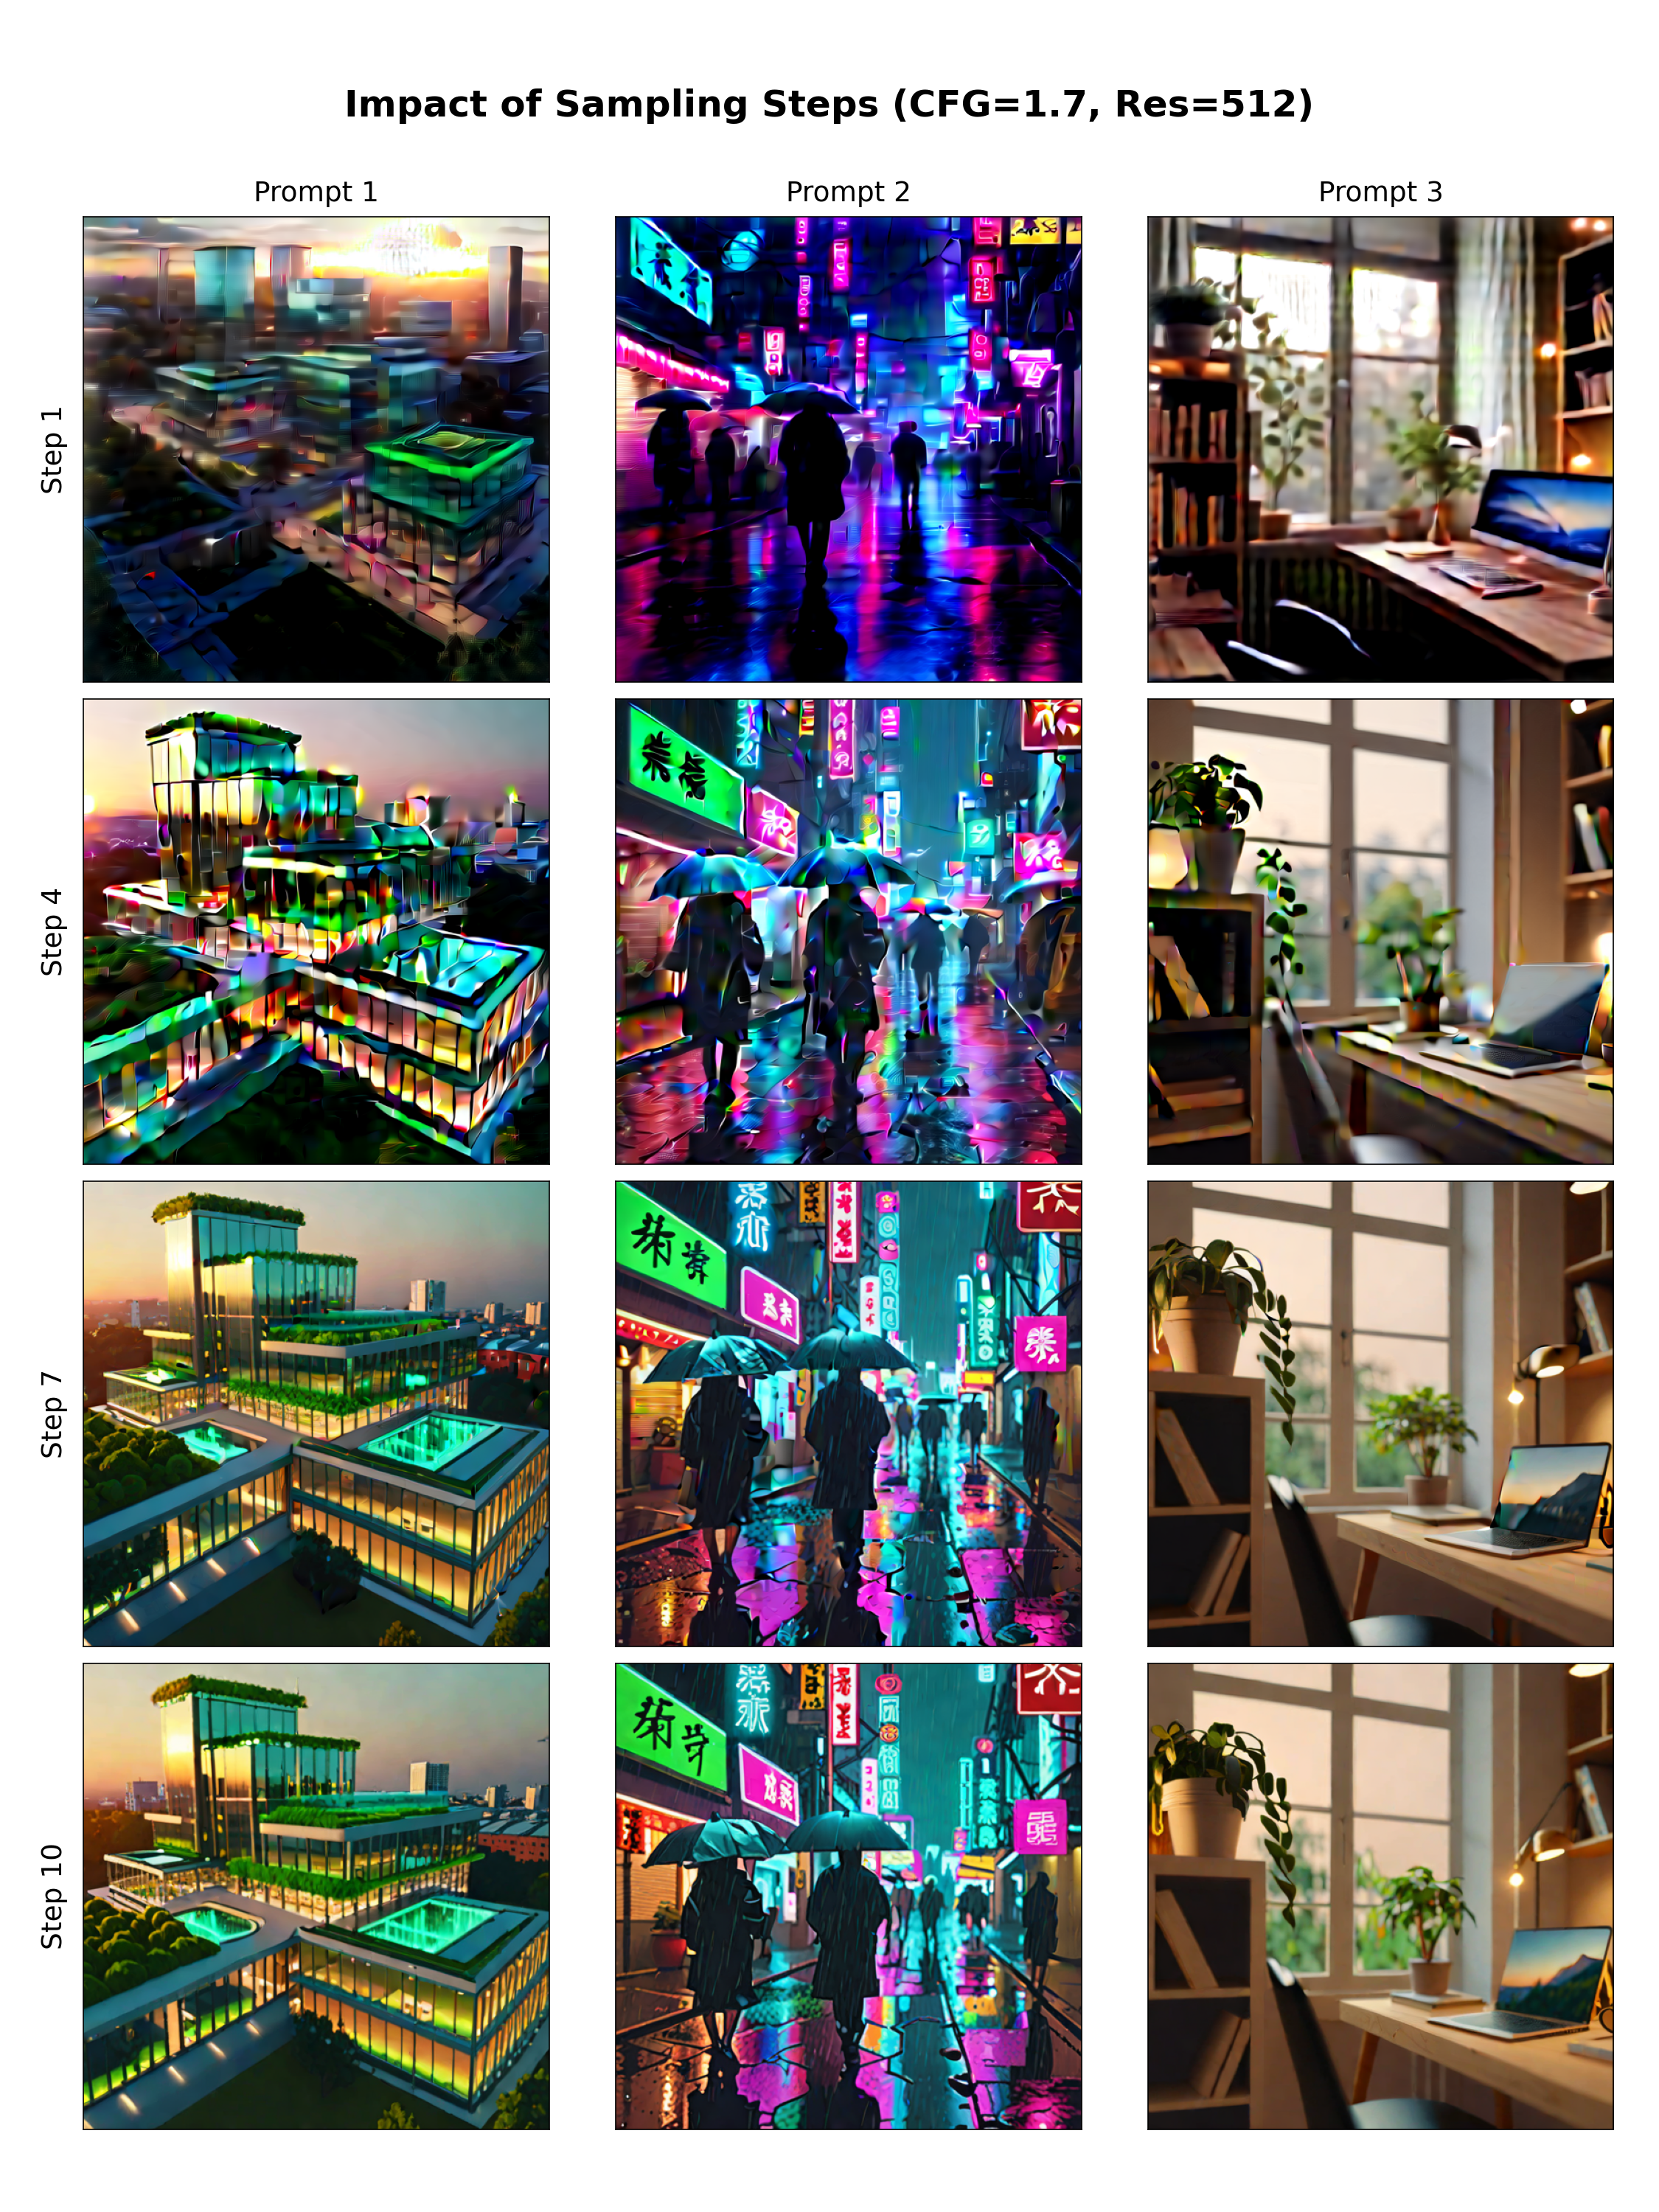
\includegraphics[width=0.5\textwidth]{comparison_steps.png}
    \caption{不同采样步数下的生成效果对比 (CFG=1.7, Res=512)。随着步数增加,图像从噪声逐渐收敛为清晰的语义场景。}
    \label{fig:steps_comparison}
\end{figure}

从整体视觉效果来看,随着采样步数的增加,图像经历了从混沌噪声到具象结构,再到精细纹理的显著变化过程。这一过程在 Prompt 2(中间列,赛博朋克风格街道)的生成结果中表现得尤为典型:

\begin{itemize}
    \item \textbf{Step 1(模糊色块阶段):} 模型尚未完成基本的去噪任务,输出结果仅为模糊的色块堆叠。我们可以看到大致的色彩分布(如霓虹灯的紫红色与青色),但完全无法辨认具体的几何结构或物体轮廓。
    
    \item \textbf{Step 4(轮廓涌现阶段):} 图像的低频信息开始确立,基本的场景结构浮现。街道的透视关系和行人的体态轮廓初步形成,但画面依然充满了噪点和不自然的伪影,细节极其粗糙,物体表面缺乏真实的材质感。
    
    \item \textbf{Step 7(细节细化阶段):} 图像质量发生质的飞跃。模糊的光斑转化为了具体的物体,特别是街道两侧的\textbf{店铺和广告牌},其边缘变得清晰锐利。原本无法辨识的霓虹灯光此时已能呈现出具体的形状,地面的积水反射也展现出了正确的光学特性。
    
    \item \textbf{Step 10(纹理真实阶段):} 画面细节进一步丰富,纹理更加真实。观察画面上方的广告牌,不仅文字符号(如汉字部分)变得清晰可辨,而且招牌的材质光泽和灯管的亮度层次也更加细腻。店铺内部的陈设细节开始显现,整体场景的立体感和真实感达到了较高水平。
\end{itemize}

分析得出,增加采样步数能够显著降低生成图像的不确定性,使模型能够逐步填充高频细节,将模糊的潜在语义转化为具有真实纹理和清晰边缘的高质量图像。对于 SDXL 模型而言,在 10 步左右即可获得结构完整且细节丰富的图像,体现了其高效的生成能力。
\subsubsection{提示词引导系数 (CFG Scale) 对生成结果的影响}

提示词引导系数(CFG Scale)用于调节模型在“自由创造”与“严格遵循提示词”之间的平衡。本实验在固定采样步数为 10、分辨率为 $512 \times 512$ 的条件下,测试了 CFG 从 1.7 到 12.0 的变化,旨在寻找最佳的参数区间。实验结果如图 \ref{fig:cfg_comparison} 所示。

\begin{figure}[h]
    \centering
    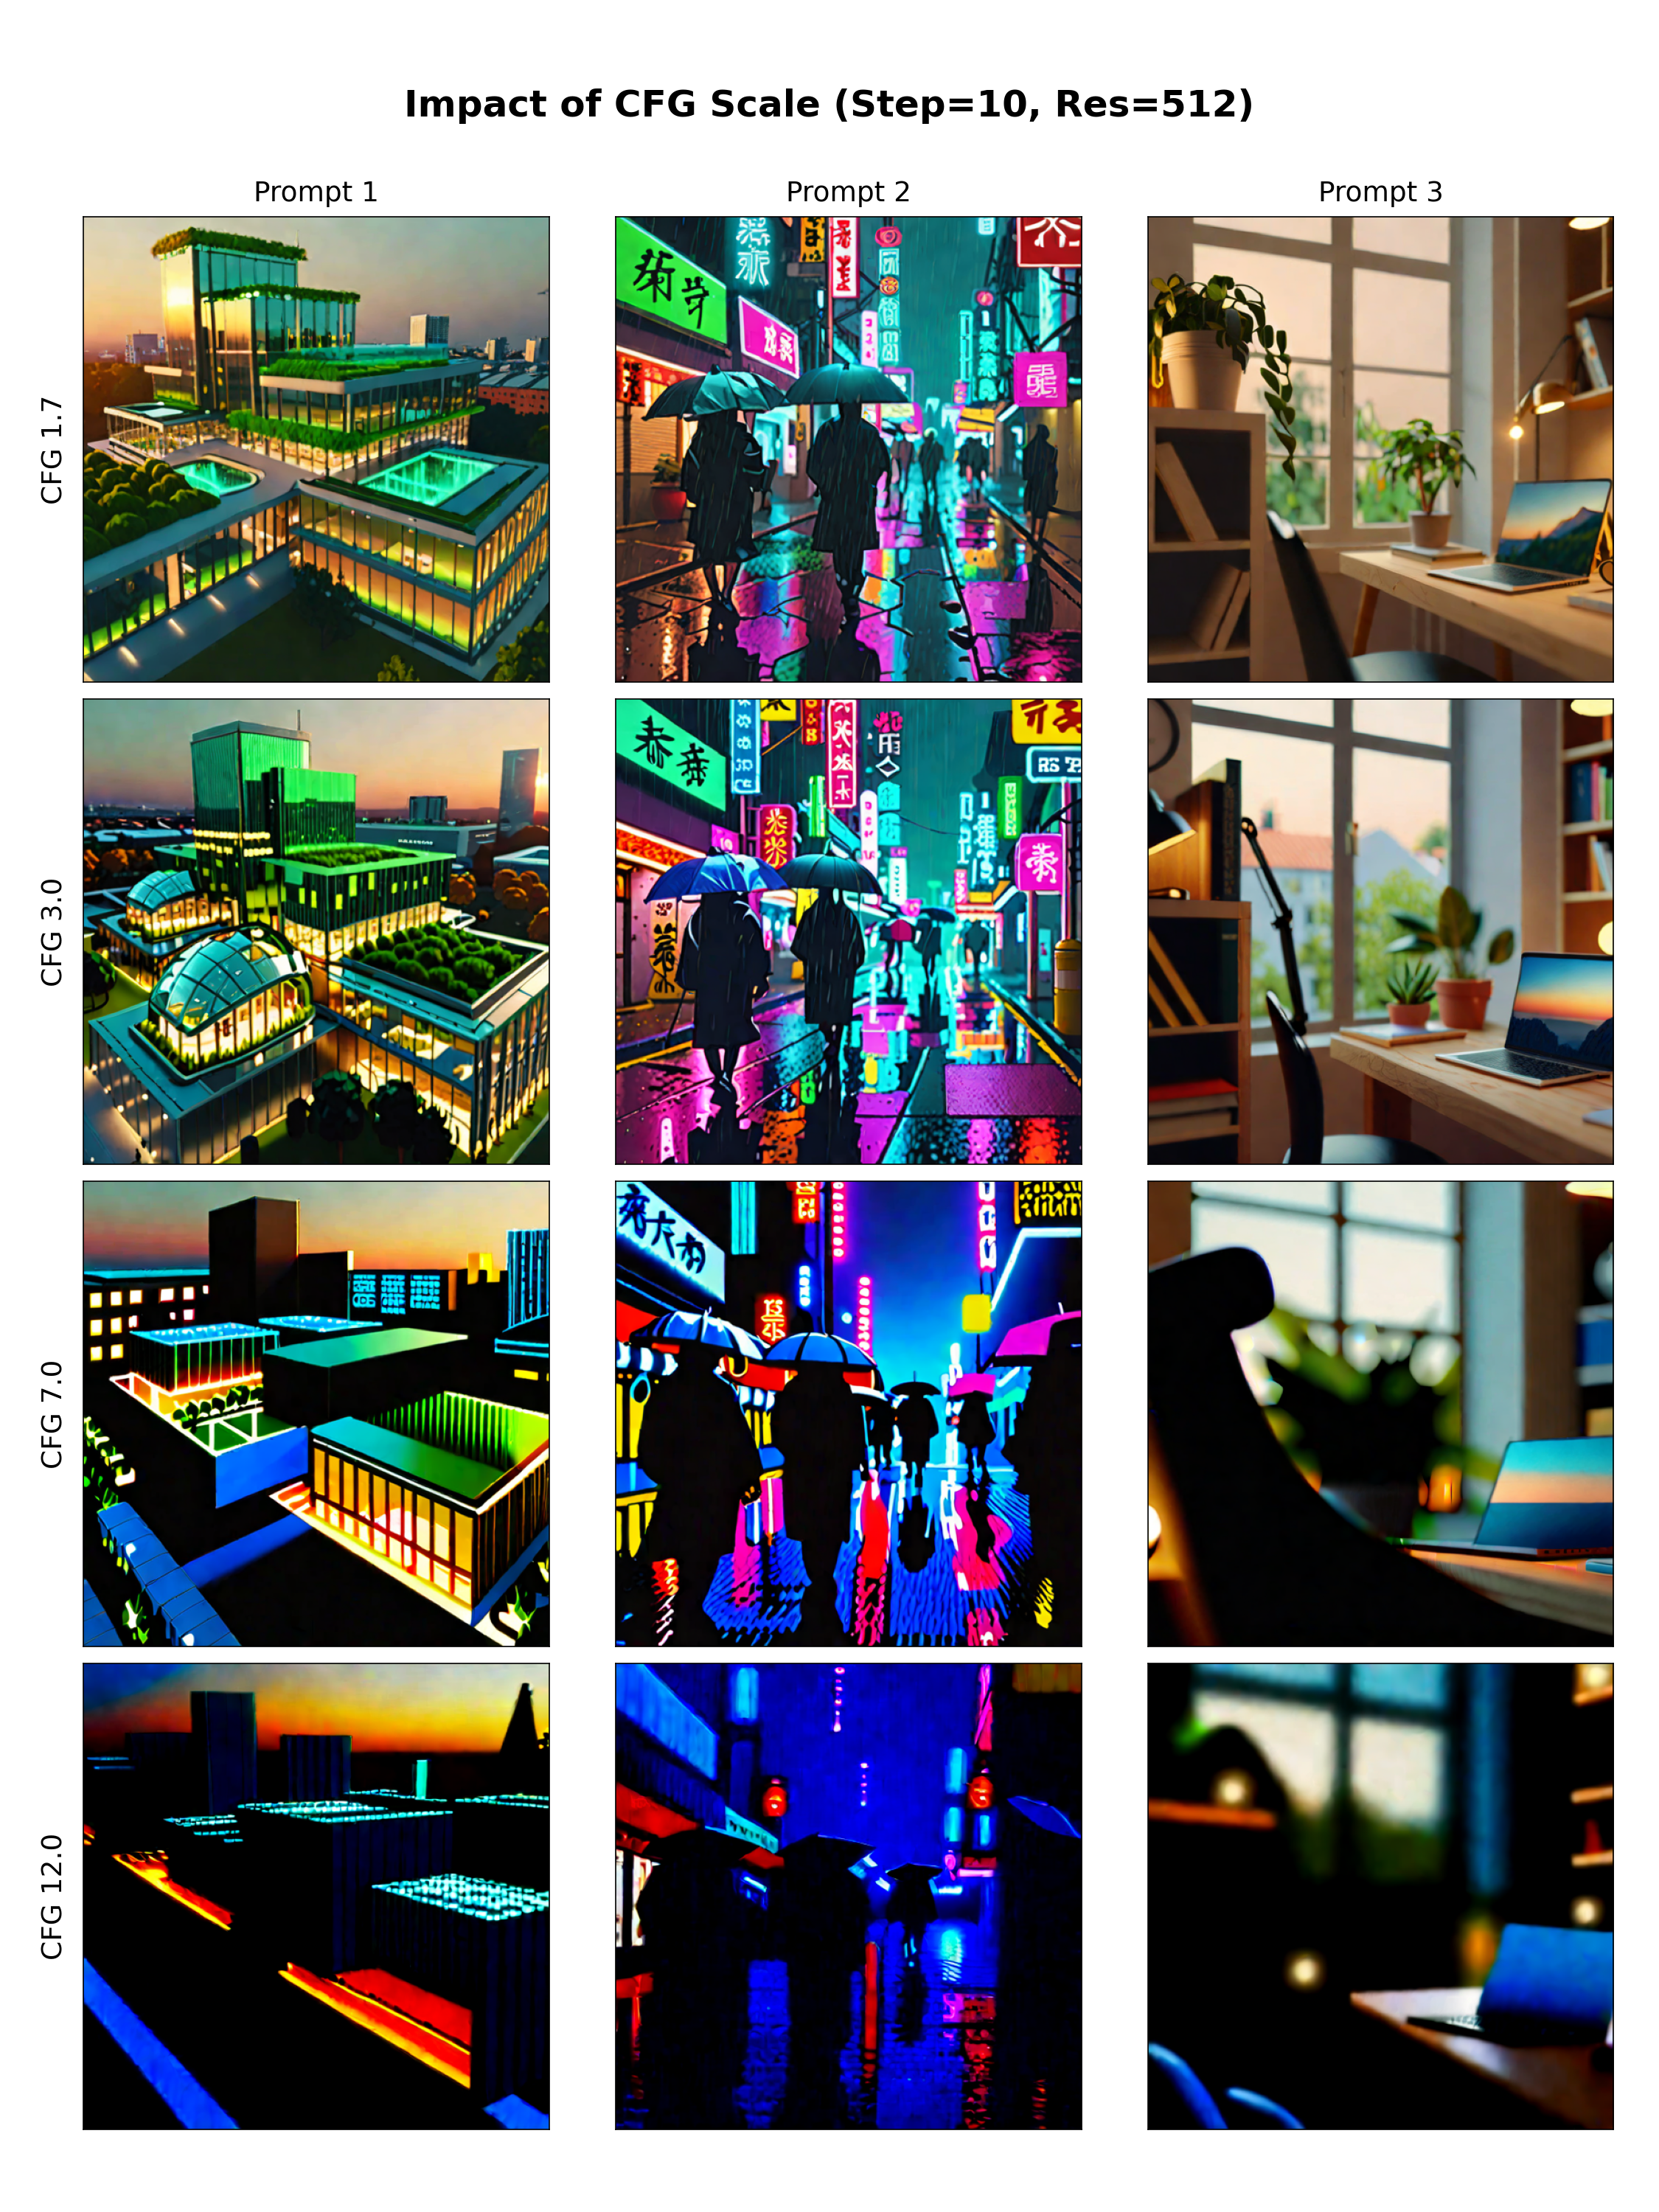
\includegraphics[width=0.5\textwidth]{comparison_cfg.png}
    \caption{不同 CFG Scale 下的生成效果对比 (Step=10, Res=512)。CFG 3.0 在保持画面自然度的同时,展现了最佳的结构清晰度。}
    \label{fig:cfg_comparison}
\end{figure}

从生成结果的演变过程可以看出:

\begin{itemize}
    \item \textbf{CFG 1.7(自然柔和):} 画面整体色调平和,光影过渡非常自然。模型享有较高的创意自由度,但在某些具体特征(如建筑的边缘锐度、室内的陈设细节)上表现得较为松散,视觉冲击力较弱。
    
    \item \textbf{CFG 3.0(最佳平衡):} \textbf{这是本组实验中表现最佳的设置。}在此数值下,图像实现了指令依从性与画面质量的完美平衡。Prompt 1 的建筑线条变得清晰硬朗,Prompt 2 的赛博朋克霓虹灯光感恰到好处,水面反光生动美观,既保留了丰富的细节,又没有出现过度的锐化,视觉观感最为舒适。
    
    \item \textbf{CFG 7.0(过度饱和):} 随着引导系数过高,画面开始出现负面效果。图像对比度和饱和度急剧增加,导致暗部细节丢失(如街道场景变得极黑),亮部出现不自然的伪影,色彩开始失真。
    
    \item \textbf{CFG 12.0(结构崩坏):} 图像结构完全崩溃。过强的强制引导破坏了潜在空间的连贯性,导致画面充斥着高对比度的噪点和无法辨识的色块,完全失去了可用性。
\end{itemize}

可以得出,对于当前的 SDXL 工作流,\textbf{CFG 3.0 左右}是理想的参数选择。它能够有效地执行文本指令,同时避免高 CFG 值带来的色彩溢出和结构崩坏问题。

\subsubsection{图像分辨率 (Resolution) 对生成结果的影响}

图像分辨率决定了生成图像的像素尺寸和画布大小。由于 SDXL 等扩散模型通常是在特定的分辨率(如 $1024 \times 1024$)上进行训练的,偏离这一“原生分辨率”过远会对生成对象的结构和构图产生显著影响。本实验在固定采样步数为 10、CFG 为 1.7 的条件下,测试了从 $512 \times 512$ 到 $2048 \times 2048$ 的四种分辨率。实验结果如图 \ref{fig:res_comparison} 所示。

\begin{figure}[h]
    \centering
    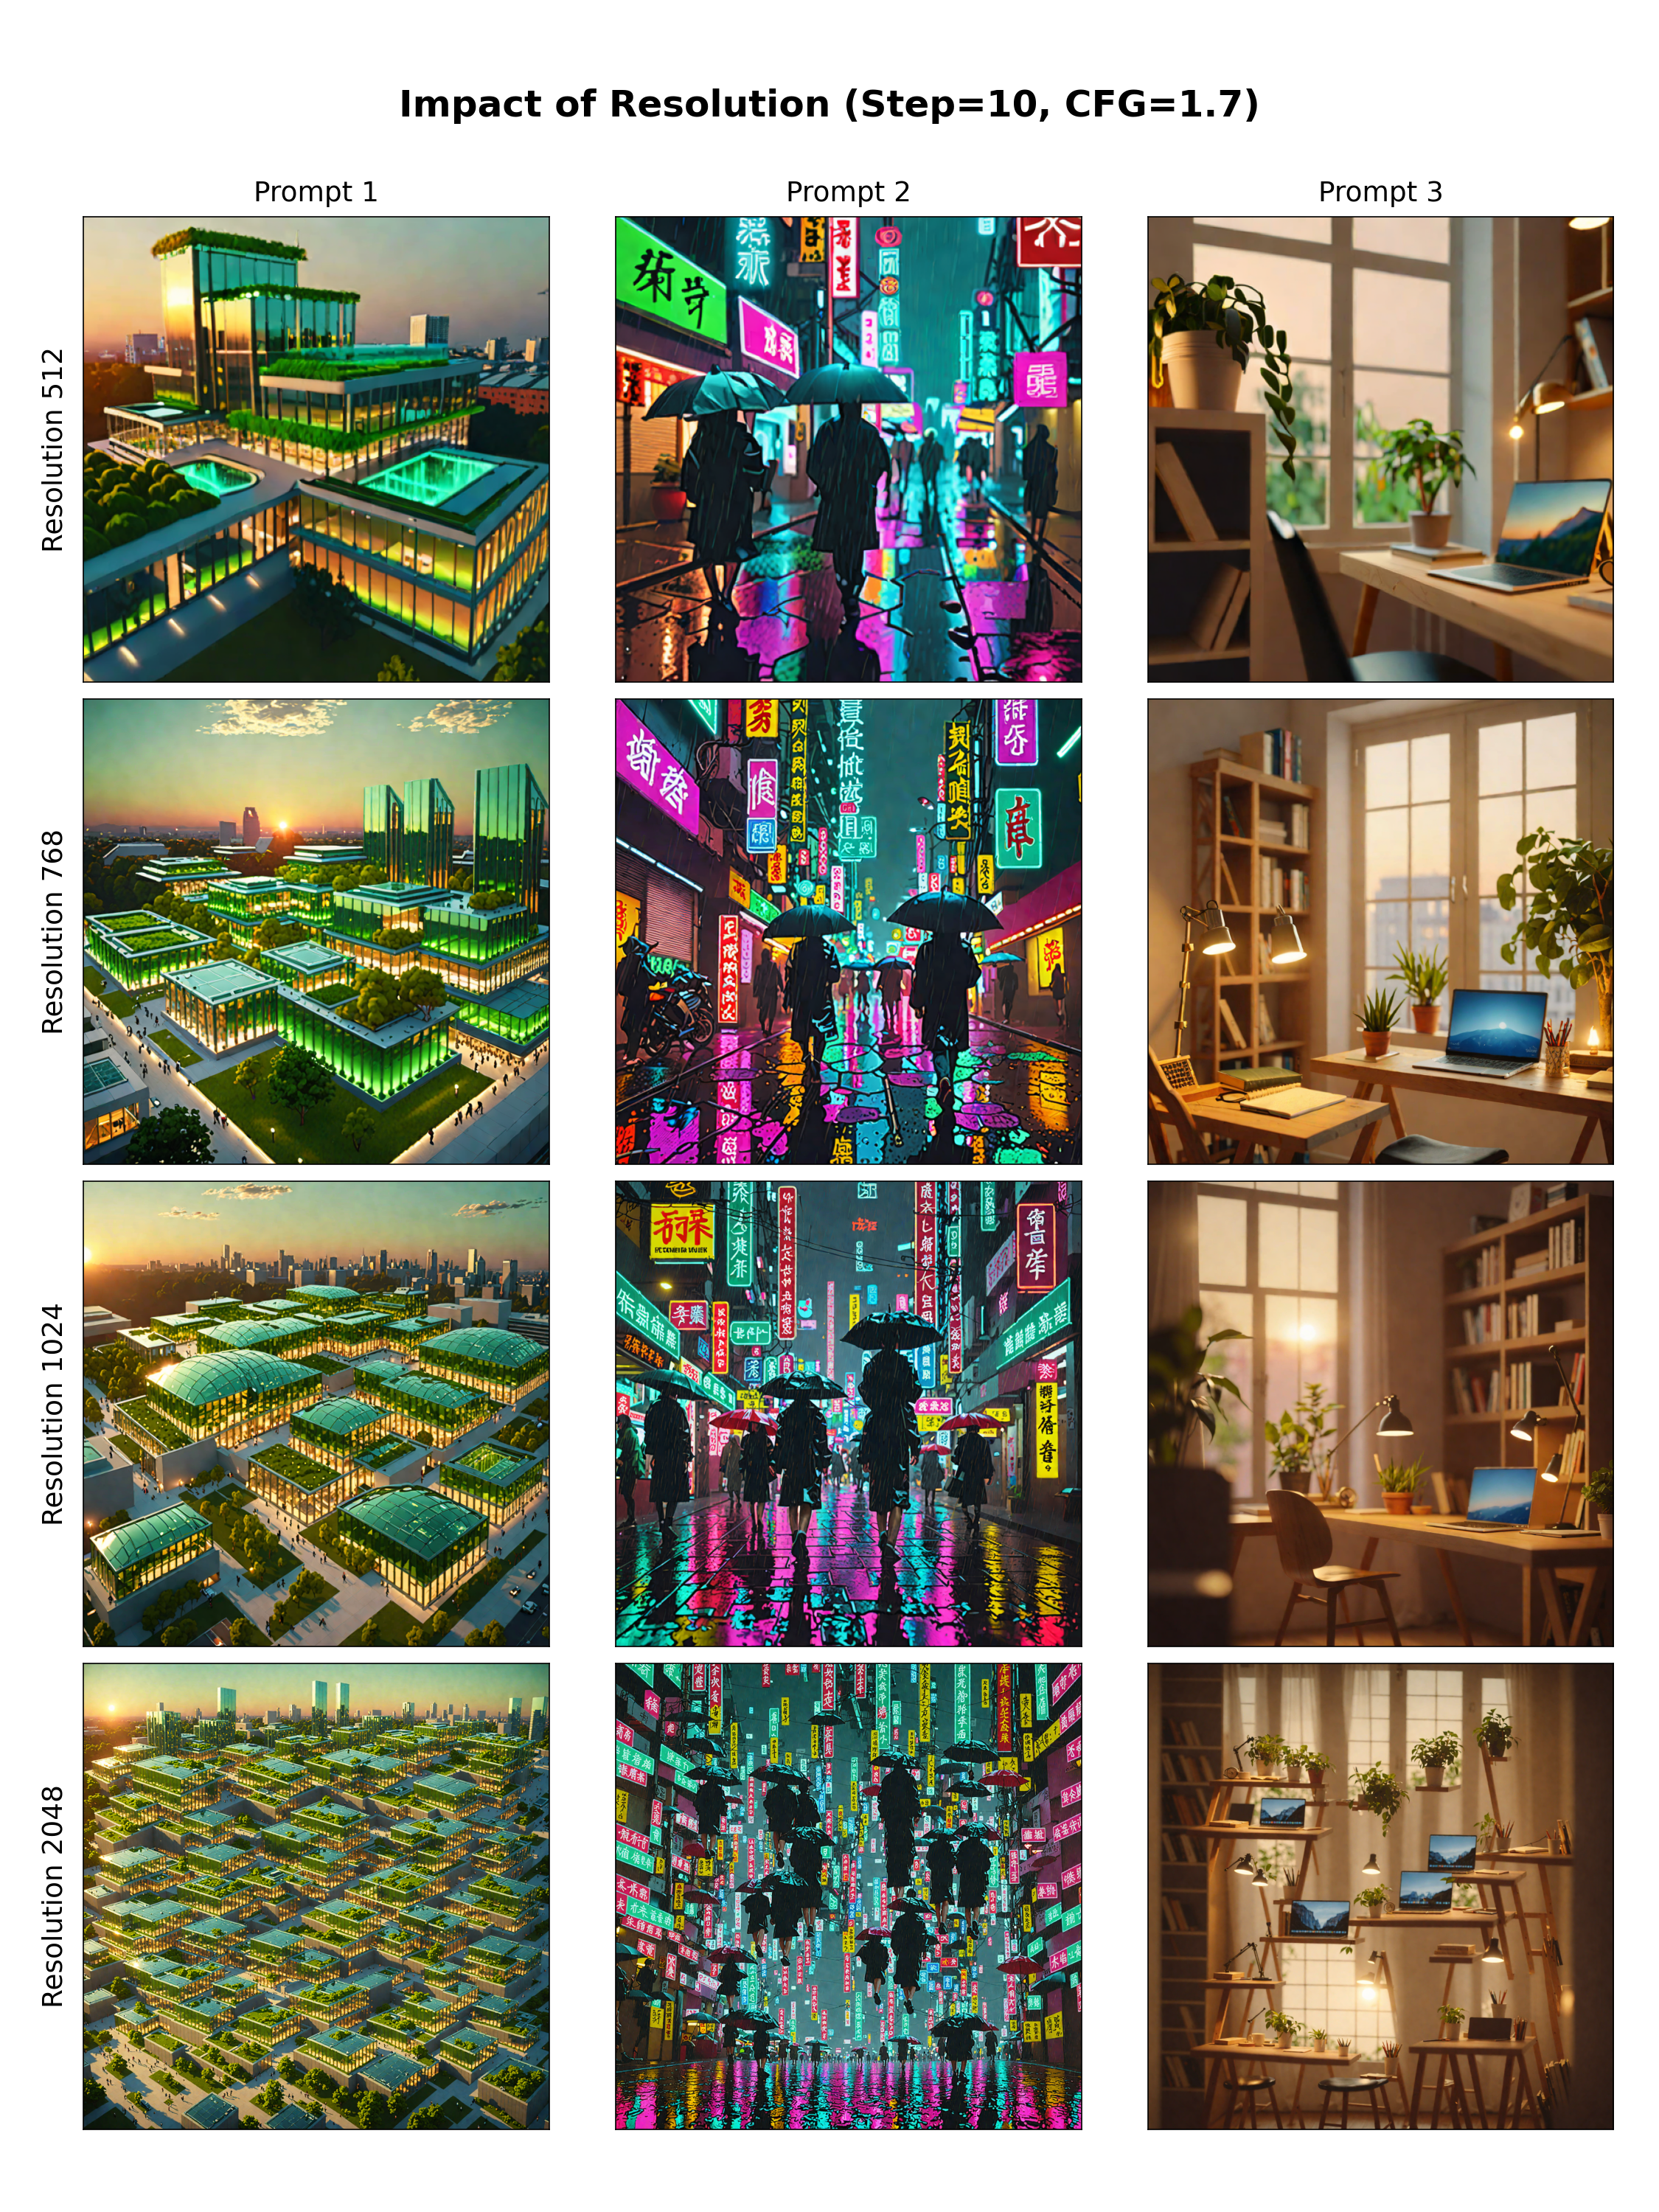
\includegraphics[width=0.5\textwidth]{comparison_resolution.png}
    \caption{不同分辨率下的生成效果对比 (Step=10, CFG=1.7)。展示了从低分辨率的模糊紧凑,到中分辨率的细节丰富,再到高分辨率下的结构崩坏与重复伪影。}
    \label{fig:res_comparison}
\end{figure}

观察不同分辨率下的生成表现,可以总结出以下规律:

\begin{itemize}
    \item \textbf{低分辨率 ($512 \times 512$) —— 内容受限与细节模糊:} 
    在此分辨率下,由于像素总量较少,模型能够承载的信息密度有限。
    \begin{itemize}
        \item \textbf{构图局促:} Prompt 1 的建筑场景仅能呈现局部,缺乏宏大的空间感。
        \item \textbf{细节缺失:} Prompt 2 的赛博朋克街道中,远处的霓虹灯牌模糊不清,人物轮廓较为粗糙,整体画面偏向于色块堆叠而非精细绘画。
    \end{itemize}
    
    \item \textbf{中等分辨率 ($768 \times 768$ 至 $1024 \times 1024$) —— 最佳生成区间:} 
    这是 SDXL 模型的最佳工作区间。随着分辨率提升至 1024,画面的清晰度和构图合理性达到峰值。
    \begin{itemize}
        \item \textbf{细节丰富:} Prompt 3 的室内场景中,书架上的书籍、桌面的摆件以及窗外的光影都得到了细腻的刻画。
        \item \textbf{结构合理:} Prompt 1 的建筑群落布局更加完整,透视关系准确,展现了高质量的生成能力。
    \end{itemize}
    
    \item \textbf{超高分辨率 ($2048 \times 2048$) —— 重复伪影与物理逻辑崩坏:} 
    当分辨率显著超出模型的训练分布时,生成质量并未随像素增加而提升,反而出现了严重的结构性错误。由于模型无法在这个尺度上维持单一对象的全局一致性,它倾向于通过“平铺”局部特征来填充画布:
    \begin{itemize}
        \item \textbf{机械重复:} 在 Prompt 1 中,建筑不再是合理的楼宇结构,而是变成了无数绿色屋顶的机械复制与堆砌,看起来更像是纹理贴图而非真实场景。
        \item \textbf{违反物理规则:} 在 Prompt 2 的街道场景中,出现了严重的逻辑谬误。人物悬浮在半空中,画面中甚至出现了多重地平线或上下颠倒的倒影,完全打破了透视学和物理学的基本规律。
    \end{itemize}
\end{itemize}

综上所述,盲目提高分辨率并不能带来画质的直接提升。SDXL 模型在接近其训练分辨率($1024 \times 1024$)时表现最佳;过低的分辨率会导致细节丢失,而过高的分辨率则会引发严重的语义重复和逻辑崩坏。

\subsection{FLUX.1 Kontext Dev 图像到图像编辑}

本章聚焦于 Task 2 图像编辑任务中的参数调控机制。鉴于\textbf{采样步数(Steps)}、\textbf{分辨率(Resolution)}以及\textbf{随机种子(Seed)}等基础生成参数已在前一章基于 SDXL 的文生图任务中进行了详尽的敏感性分析,本节将不再对这些通用变量产生的常规影响进行重复赘述。

为了验证 FLUX.1 Kontext Dev 模型在多模态编辑中的可控性与灵活性,并针对图生图(Image-to-Image)任务的特异性,我们在本实验中将核心关注点收束于以下几组决定生成行为与编辑质量的关键参数:

\begin{itemize}
    \item \textbf{Flux 引导 (Flux Guidance):} 
    这是 FLUX.1 架构特有的核心参数(截图中设定为 2.5)。区别于前一章讨论的常规 CFG Scale,该参数在 FLUX 模型中专门用于调节生成图像的风格倾向与指令遵循度。较低的数值(如实验设定的 2.5)有助于生成更加写实、自然的摄影风格图像,而较高的数值则会强化图像的锐度与风格化特征。
    
    \item \textbf{采样算法与调度策略 (Sampler \& Scheduler):} 
    采样器(Sampler)是决定扩散模型生成质量、推理速度以及最终图像风格的核心数学引擎,它负责计算潜在空间中每一步的更新方向。配合负责控制噪声移除速率与算法逻辑的调度器(Scheduler),两者共同决定了图像从噪声重构为清晰图像的具体路径。
    
    在本实验中,为了探究不同采样策略对 FLUX.1 模型编辑性能的影响,我们将保持调度器为 \textbf{simple} 不变,重点对比以下三种具有代表性的采样算法:
    \begin{enumerate}
        \item \textbf{Euler:} 经典的数值微分方程求解算法,通常作为 FLUX 模型的默认基准(Baseline),在生成速度与图像质量之间保持着良好的平衡。
        \item \textbf{DDPM~\cite{ddpm}:} 最原始的去噪扩散概率模型算法,理论上能提供极高的生成质量与细节还原,但通常推理速度较慢。
        \item \textbf{LCM~\cite{lcm} (Latent Consistency Models):} 专为加速生成而设计的蒸馏算法,旨在通过极少的采样步数实现快速收敛,重点测试其在实时编辑场景下的潜力。
    \end{enumerate}
    
    \item \textbf{降噪强度 (Denoising Strength):} 
    这是图生图(Image-to-Image)工作流中控制“重绘幅度”的最关键变量(默认 KSampler 为 1.00)。该参数定义了模型在生成过程中对原始输入图像的修改程度:数值越低,原图的结构与细节保留得越完整;数值越高(趋近于 1.00),模型则获得更大的自由度对图像进行重构。在编辑任务中,调节此参数是平衡“维持原貌”与“执行修改”的主要手段。
\end{itemize}

\subsubsection{Flux 引导系数 (Flux Guidance) 对生成细节与风格的影响}

通过对比不同 Flux 引导系数(1.0, 2.5, 4.0)下的生成结果,我们可以清晰地观察到该参数在提升图像创意性、丰富细节以及增强光影真实感方面的关键作用。具体效果如图 \ref{fig:flux_guidance} 所示。

\begin{figure}[htbp]
    \centering
    % 请确认文件名后缀是 .jpg 还是 .png,并确保图片在当前路径下
    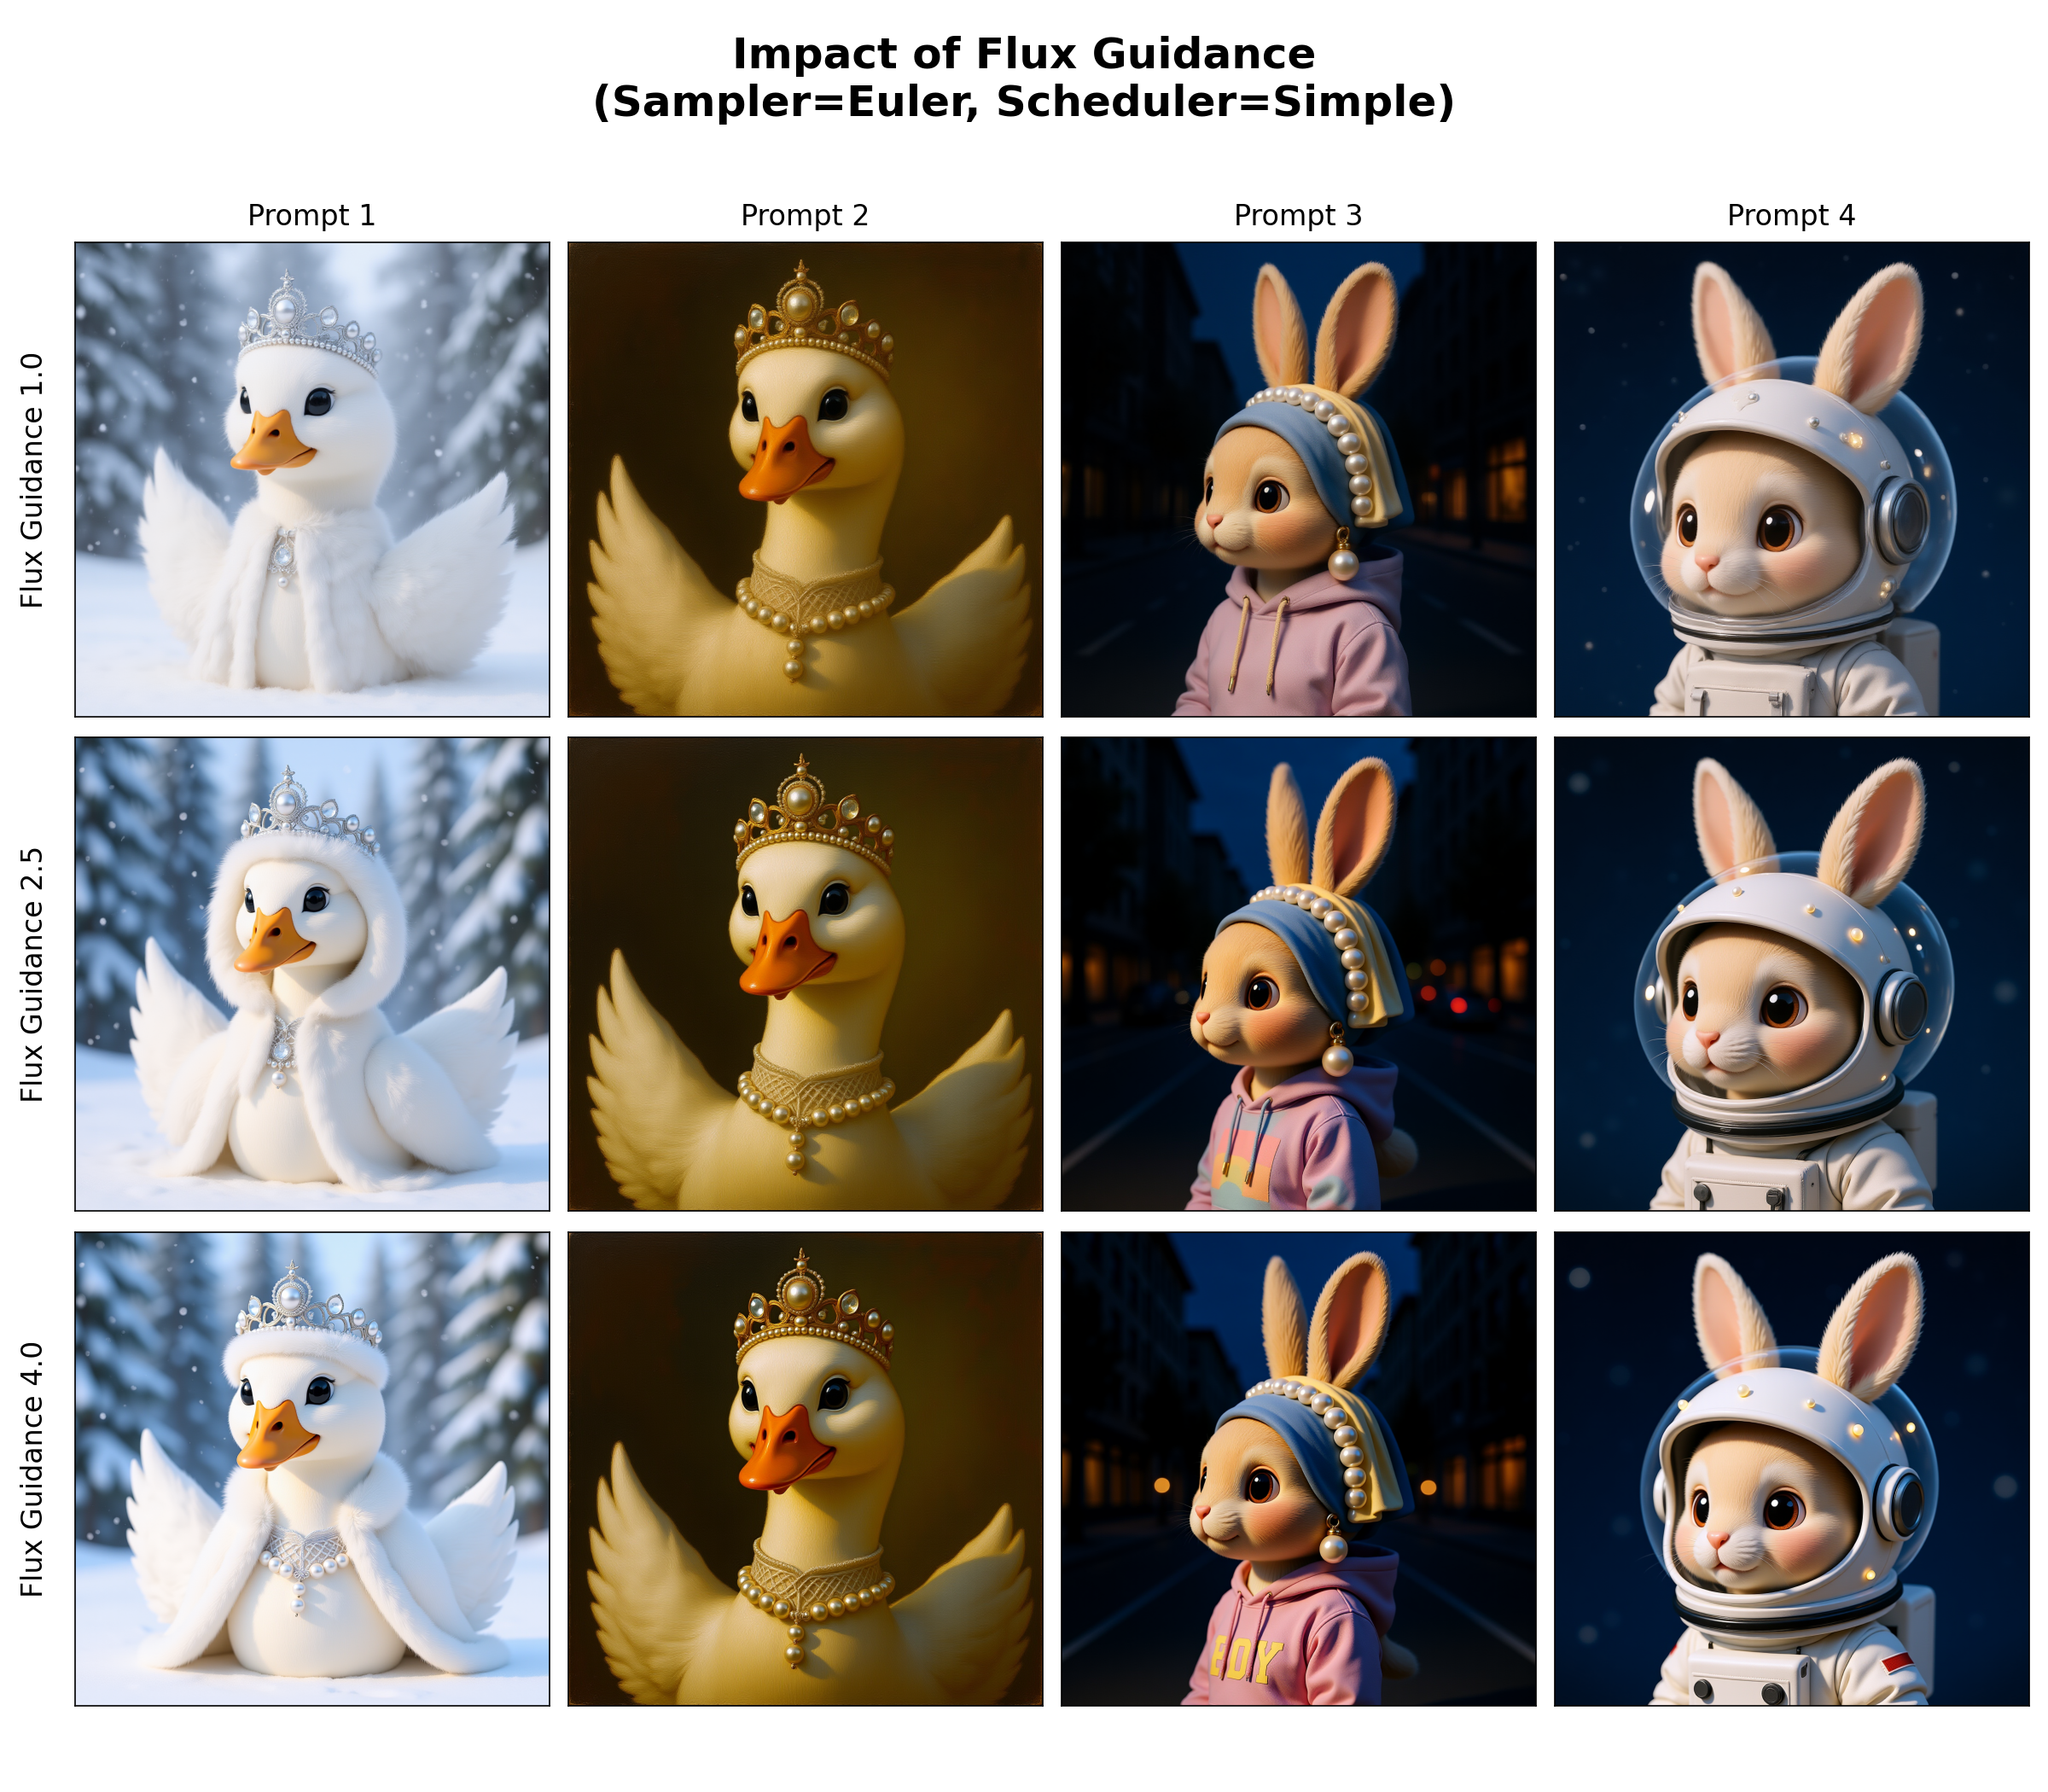
\includegraphics[width=0.5\textwidth]{flux_guidance_comparison.png}
    \caption{不同 Flux 引导系数下的生成效果对比。随着数值提升,Prompt 3 中的服饰增加了 Logo 与纹理细节,Prompt 1 的外套结构也演变得更为复杂(如增加兜帽),光影立体感显著增强。}
    \label{fig:flux_guidance}
\end{figure}

这一趋势在 Prompt 3(兔公主)的生成结果中表现得尤为显著。
\begin{itemize}
    \item \textbf{细节丰富度与创意性:} 在低引导值(Flux 1.0)下,兔公主穿着一件纯色的粉色连帽衫,视觉元素较为单一。随着引导系数的提升,服装细节发生了明显的演变:在 Flux 4.0 时,卫衣上不再是单调的纯色,而是出现了清晰的 Logo 印花与复杂的图案设计。这表明较高的引导值能激发模型生成更多的语义细节,赋予图像更强的叙事感。
    \item \textbf{光影真实感:} 随着参数增大,光影渲染变得更加立体和逼真。环境光在兔公主面部绒毛上的漫反射效果在 Flux 4.0 下表现得最为细腻,明暗对比的增强使得主体与背景的分离度更高,极大地提升了画面的写实质感。
\end{itemize}

此外,Prompt 1(鸭公主)也展示了该参数对物体结构的精细控制。
我们可以观察到外套款式的具体变化:在低引导值下,服装倾向于一种简约优雅的“小香风”毛领披肩设计;而当 Flux 引导提升后,服装的结构变得更加复杂,逐渐演变为具有厚实感且带有明显\textbf{兜帽}设计的冬装外套。这进一步验证了调节 Flux 引导系数能够有效地引导模型在保持整体风格一致的同时,对画面主体的结构特征进行更具“设计感”的重构。


\subsubsection{采样算法 (Sampler) 对生成质量与逻辑一致性的影响}

为了探究采样策略在图像编辑任务中的表现,我们保持 Flux 引导系数为 2.5,调度器为 Simple,重点对比了 \textbf{Euler}、\textbf{DDPM} 和 \textbf{LCM} 三种采样算法。实验结果如图 \ref{fig:flux_sampler} 所示,三者在画面纯净度、语义逻辑和细节处理上表现出显著差异。

\begin{figure}[htbp]
    \centering
    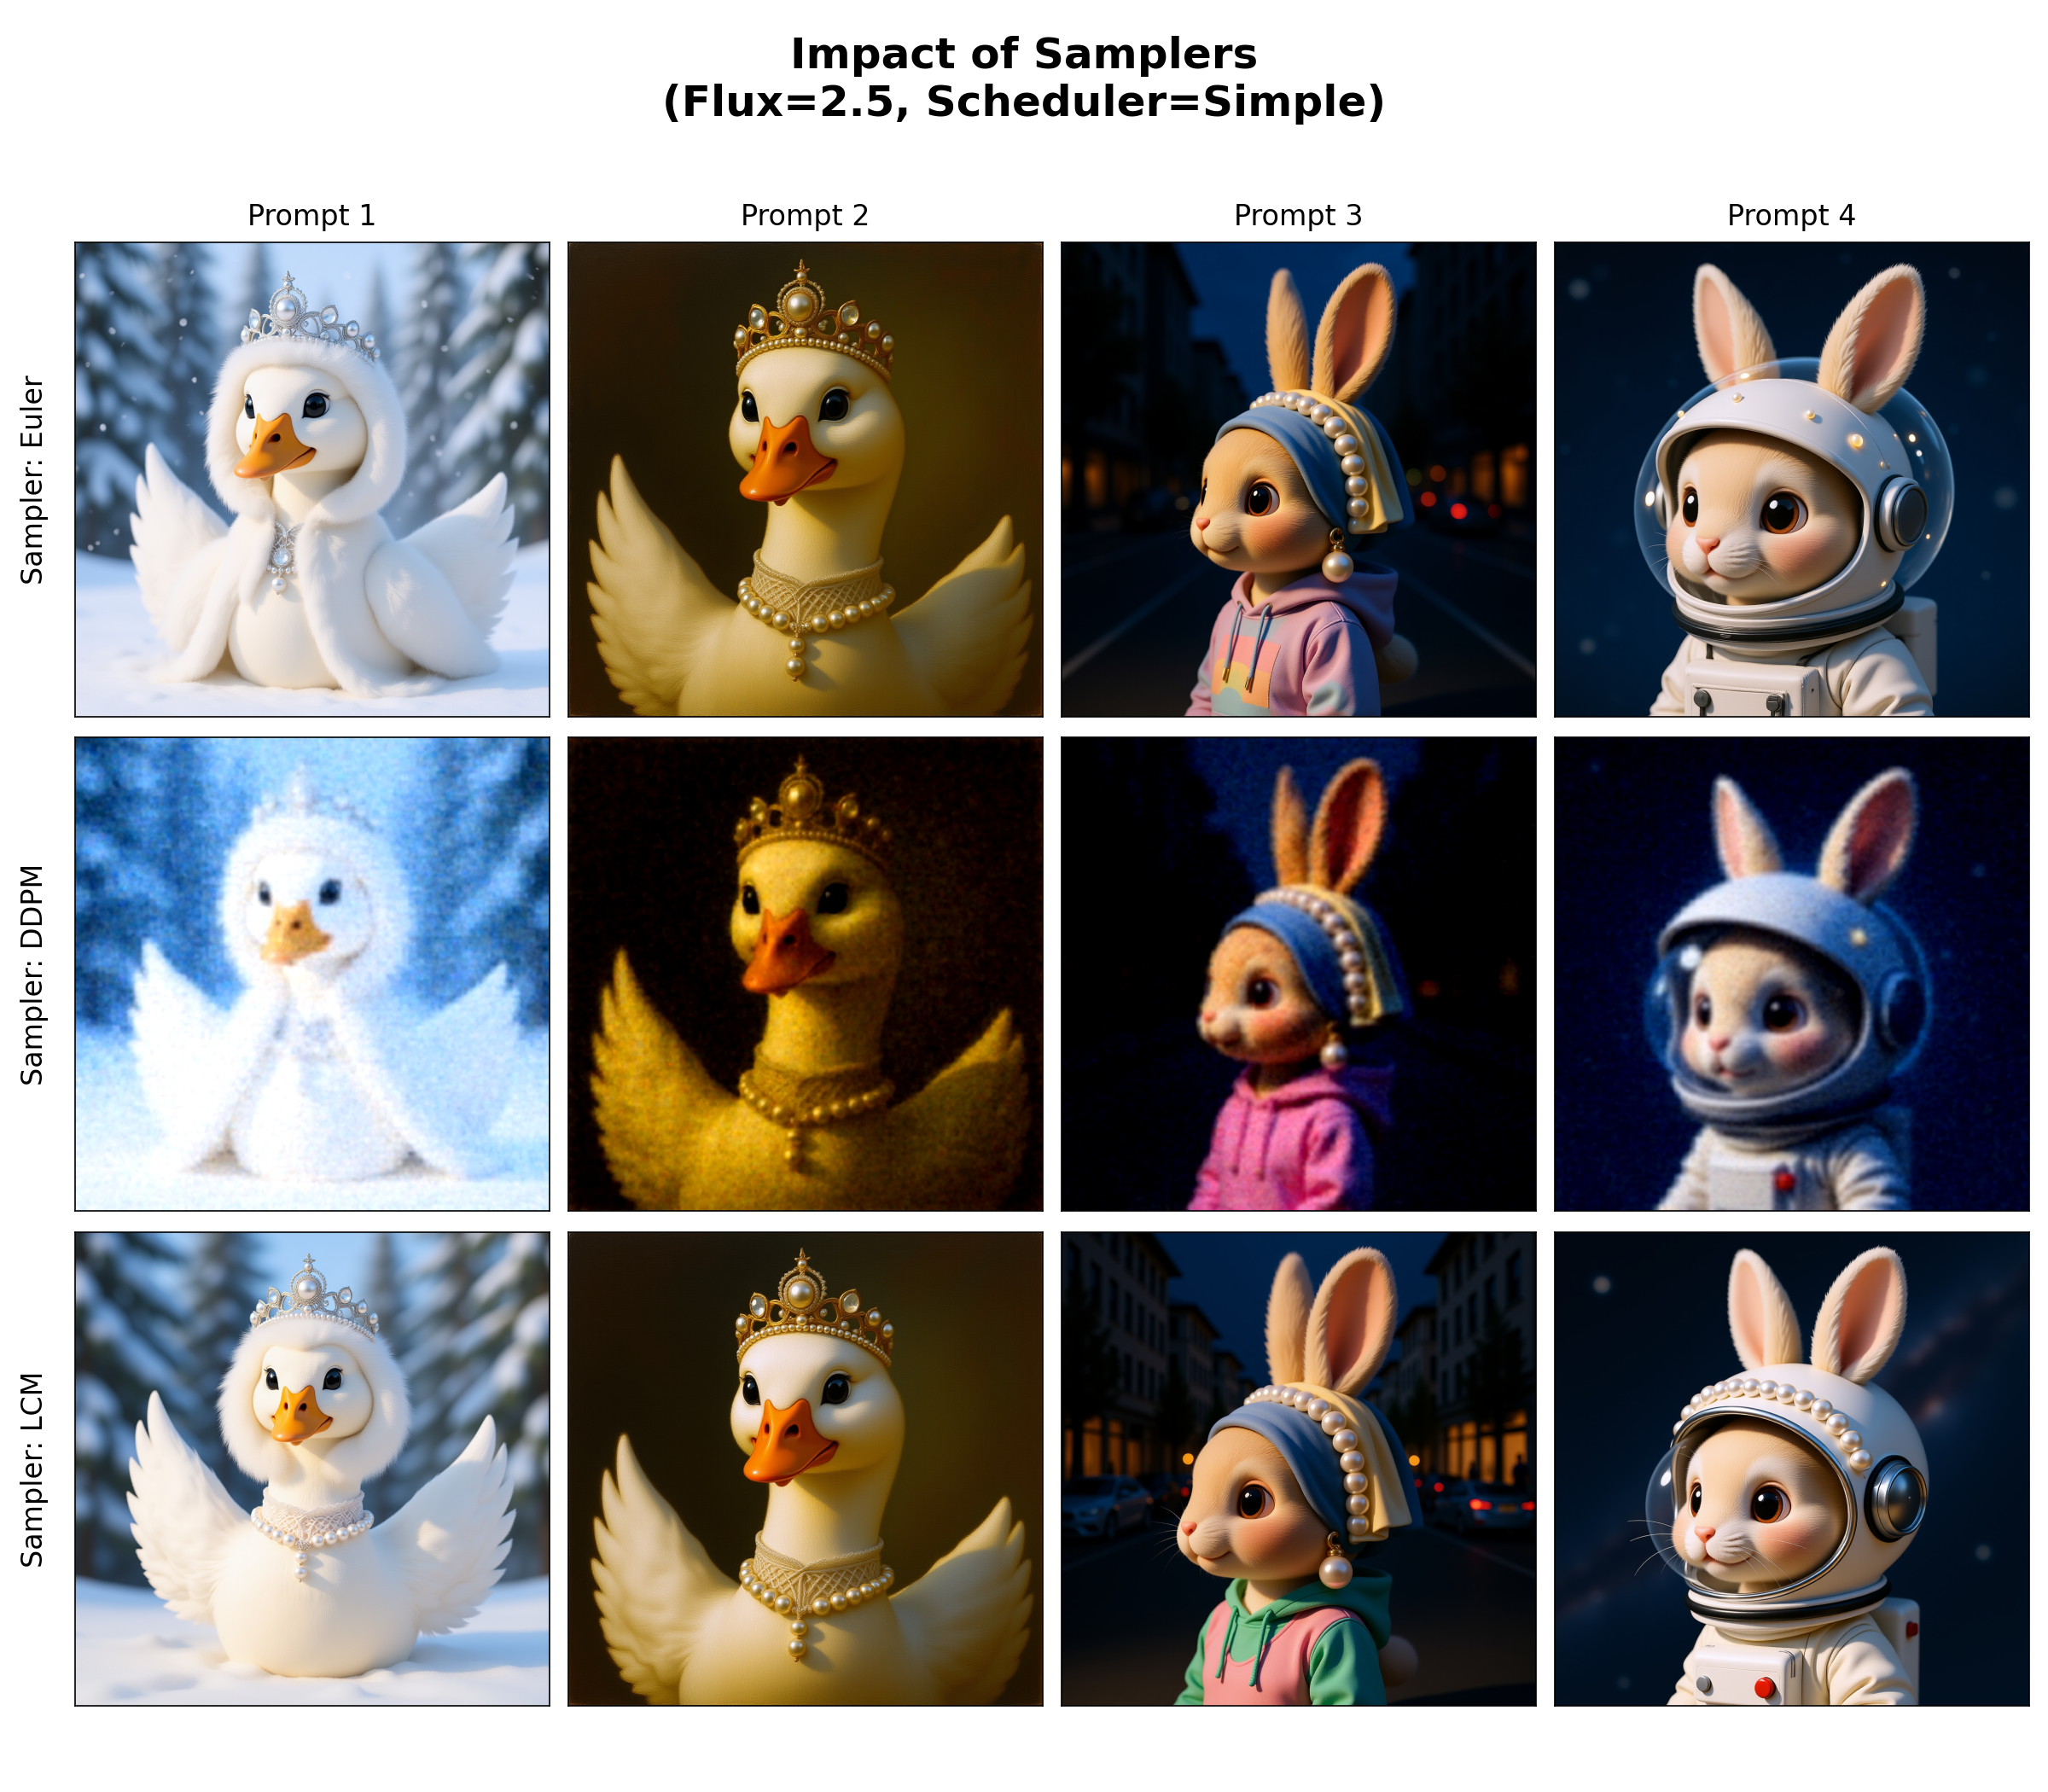
\includegraphics[width=0.5\textwidth]{flux_sampler_comparison.png}
    \caption{不同采样算法 (Sampler) 下的生成效果对比。DDPM 因步数不足导致严重噪点;LCM 虽质感真实但出现了“珍珠耳环残留”等逻辑错误;Euler 展现了最佳的综合效果。}
    \label{fig:flux_sampler}
\end{figure}

\begin{itemize}
    \item \textbf{DDPM (Denoising Diffusion Probabilistic Models):} 
    作为扩散模型的经典奠基算法,DDPM 在本实验中表现最差,生成的图像充斥着大量无法去除的高频噪点,主体几乎不可辨识。
    \textbf{原因分析:} DDPM 的逆向去噪过程通常需要数百甚至上千个采样步数才能收敛至清晰图像。而在本实验设置的常规步数( 20 步)下,DDPM 算法无法完成完整的马尔可夫链去噪过程,导致中间状态的噪声大量残留。这表明标准的 DDPM 并不适合现代追求效率的短步数工作流。

    \item \textbf{LCM (Latent Consistency Models):} 
    LCM 算法展现了极强的画面表现力,其生成的图像光影对比强烈,材质的真实感甚至在某些局部超过了 Euler。然而,实验发现 LCM 在语义逻辑的重组上存在明显缺陷,表现出一种“过度拟合原特征”或语义融合的倾向:
    \begin{itemize}
        \item 在 \textbf{Prompt 1}(鸭公主)中,原本应穿在身上的白色外套被错误地处理成了包裹头部的毛绒头套,结构出现了混淆。
        \item 在 \textbf{Prompt 4}(宇航员兔公主)中,尽管场景切换到了太空,兔公主耳朵上依然保留了 Prompt 3 中的\textbf{珍珠耳环},且生硬地穿插在宇航服头盔结构中。这说明 LCM 在进行场景转换时,可能过于注重保留原始图像的局部特征(如珍珠),从而忽视了新场景(宇航服)的物理逻辑约束。
    \end{itemize}

    \item \textbf{Euler:} 
    综合来看,\textbf{Euler} 采样器在本组实验中表现最佳。它不仅生成了纯净无噪点的图像,而且在逻辑一致性上远超 LCM。在 Prompt 1 中,鸭公主的皇冠与外套层次分明;在 Prompt 4 中,兔公主宇航员的装备严谨合规,没有出现不合时宜的饰品残留。Euler 算法在保证生成质量、遵循提示词逻辑以及维持画面结构之间取得了完美的平衡,是 FLUX.1 模型最为推荐的采样选择。
\end{itemize}

\subsubsection{调度策略 (Scheduler) 对生成结果的影响与伪影分析}

在确定了 Euler 为最佳采样算法后,我们进一步固定 Flux 引导系数为 2.5,采样器为 Euler,对比了 \textbf{Simple}、\textbf{Karras} 和 \textbf{Exponential} 三种调度器(Scheduler)的表现。实验结果如图 \ref{fig:flux_scheduler} 所示,结果呈现出极端的两极分化。

\begin{figure}[htbp]
    \centering
    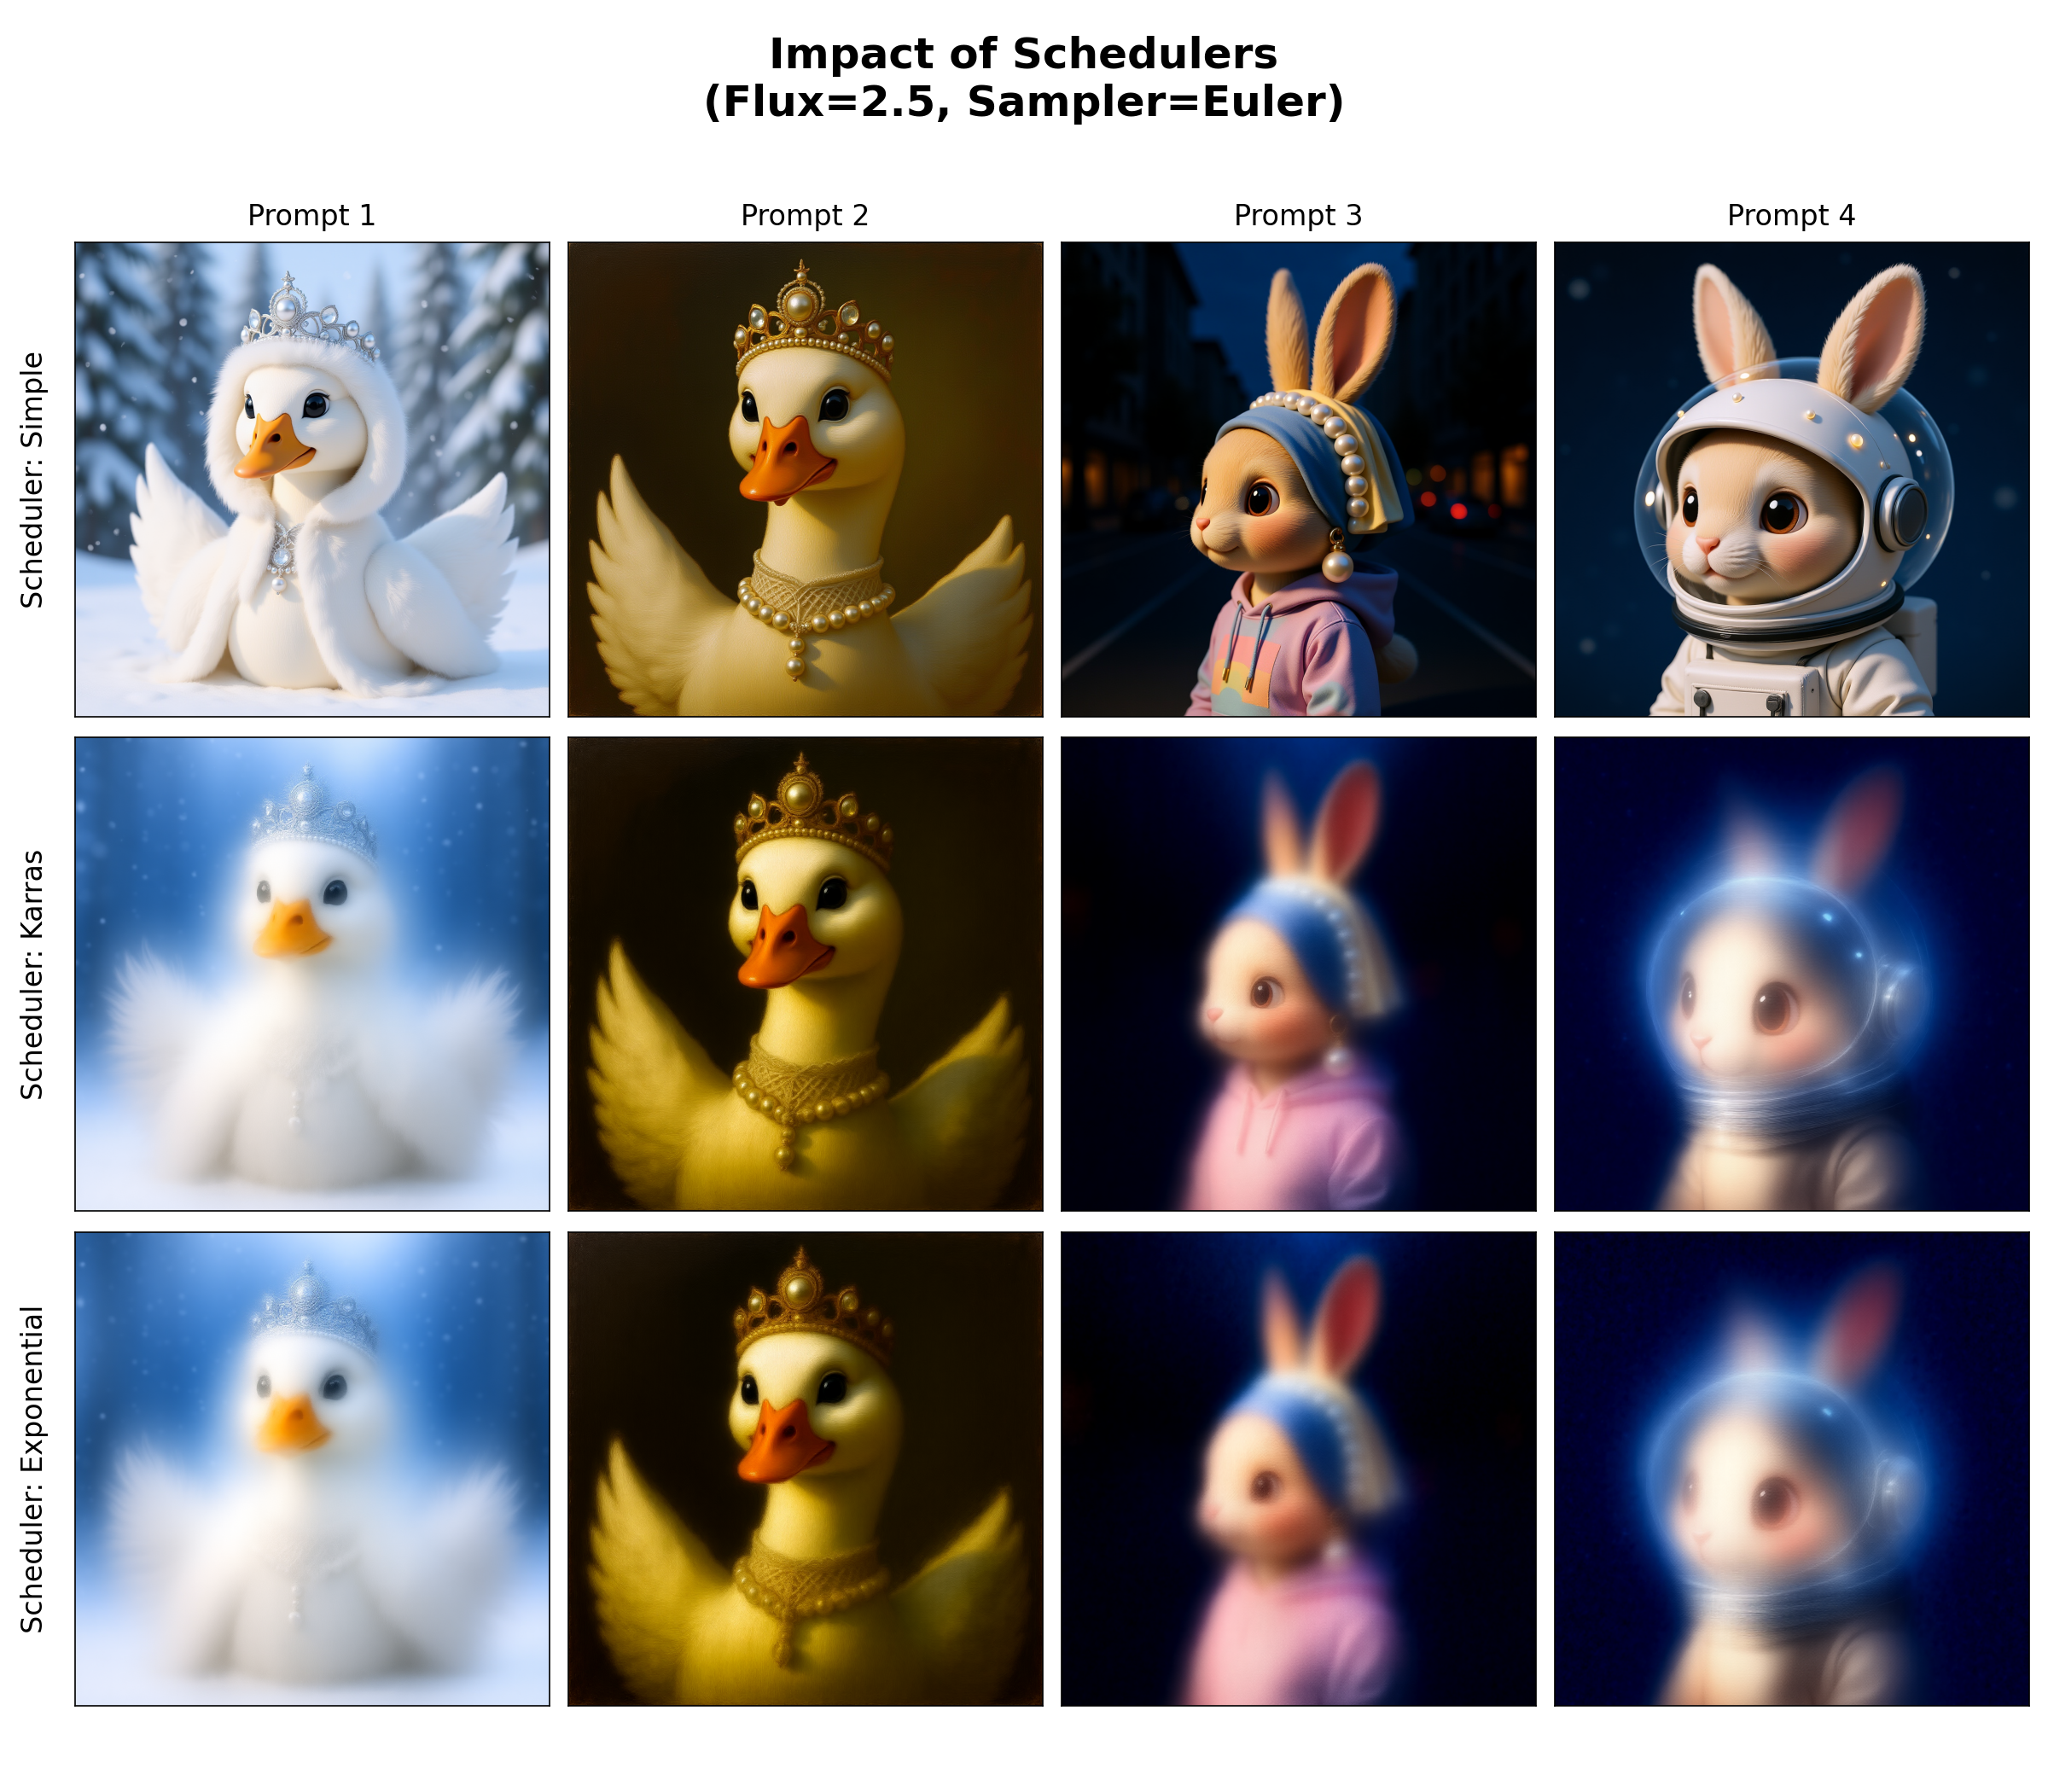
\includegraphics[width=0.5\textwidth]{flux_scheduler_comparison.png}
    \caption{不同调度器 (Scheduler) 下的生成效果对比。Simple 调度器生成了清晰的图像,而 Karras 和 Exponential 均导致了严重的模糊和细节丢失。}
    \label{fig:flux_scheduler}
\end{figure}

\begin{itemize}
    \item \textbf{Simple 调度器(最佳表现):} 
    如图第一行所示,使用 Simple 调度器生成的图像清晰锐利,纹理细节丰富(如鸭子的羽毛、兔公主的宇航服接缝)。这是因为 FLUX.1 模型是基于\textbf{流匹配(Flow Matching)}架构训练的,其底层的 Rectified Flow 技术假设噪声到数据的变换路径是线性的。\textbf{Simple} 调度器提供了一种线性的噪声衰减策略,这与 FLUX 模型的训练分布完美契合,因此能够正确地“导航”去噪过程,从噪声中还原出高清图像。

    \item \textbf{Karras 与 Exponential 调度器(严重模糊):} 
    实验显示,这两种调度器生成的结果均为严重的\textbf{高斯模糊状},图像仅保留了基本的颜色分布和模糊的轮廓(如发光的白色色块),完全丢失了高频细节。
    
    \textbf{原因分析:} 这种现象并非偶然,而是由模型架构与调度策略的\textbf{不匹配}造成的:
    \begin{enumerate}
        \item \textbf{噪声曲线不匹配:} Karras 和 Exponential 调度器是专为传统扩散模型(如 SD1.5, SDXL)设计的,它们采用非线性的 sigma 曲线,倾向于在中间噪声水平分配更多的采样步数。
        \item \textbf{去噪路径偏离:} FLUX 模型期望的是均匀的线性去噪步长。当强行使用 Karras 或 Exponential 的非线性步长时,采样器在低噪阶段(即生成纹理细节的关键阶段)的步长分配不仅不符合模型预期,甚至可能导致采样器在错误的噪声水平上进行查询。
        \item \textbf{结果:} 这种不匹配导致模型无法有效地收敛高频信息,最终输出的图像停留在了某种“未完成”的中间潜空间状态,表现为视觉上的极度模糊和光晕感。
    \end{enumerate}
\end{itemize}

 对于 FLUX.1 等流匹配模型,\textbf{Simple}(或 Beta)是唯一推荐的调度器选择,而适用于旧版扩散模型的 Karras 和 Exponential 策略在此架构下完全不可用。

\subsubsection{FLUX.1 Kontext Dev 实验结论}
基于对 Flux 引导、采样器及调度器等关键参数的敏感性测试,本实验利用“鸭公主”与“兔公主”两组核心样本,深入评估了 FLUX.1 Kontext Dev 模型的综合编辑性能。在\textbf{基础属性修改}层面,模型展现了极高的语义响应精度与细节生成能力,这在 Prompt 3 的变体中表现尤为显著:随着引导系数的介入,模型不仅成功在兔子卫衣上增添了 Logo 印花,更精确优化了面部绒毛的光影遮蔽效果,使其质感更加逼真;同时在 Prompt 1 中,模型也准确执行了对外套结构的重构(从简约领口变为兜帽设计)。在\textbf{风格迁移}与\textbf{角色一致性}方面,FLUX.1 表现出卓越的特征解耦能力:它不仅精准区分了 Prompt 2 的古典油画质感与 Prompt 4 的 3D 写实风格,更在场景发生剧烈切换(如从街头穿越至太空)时,在 Euler 采样器的配合下完美锁定了角色的面部生物特征与神态,避免了主体身份的漂移。需要指出的是,由于实验中降噪强度(Denoising Strength)在 0.95-1.00 高阈值区间表现出“完全保留原图”或“完全重绘失效”的两极化特性,缺乏分析价值,故不再赘述;同时因测试用例未包含文字编辑指令,相关能力亦不在此次评估范围内。


%%%%%%%%%%%%%%%%%%%%%%%%%%%%%%%%%%%%%%%%%%%%%%%%%%%%%%%%%%%%%%%%%%%%%%
% 实验部分(已替换为占位符)
%%%%%%%%%%%%%%%%%%%%%%%%%%%%%%%%%%%%%%%%%%%%%%%%%%%%%%%%%%%%%%%%%%%%%%
% \section{实验结果与分析}\label{sec:Experiment}

% 我们在本节中展示实验设置、数据集介绍以及定性和定量的对比结果。

% \subsection{实验设置}
% \mypara{数据集} 我们在以下数据集上进行了测试:Dataset A, Dataset B...
% \mypara{参数设置} 实验中使用的参数如下:$\alpha = 0.5, \beta = 0.9$...
% \mypara{评价指标} 我们使用准确率(Precision)、召回率(Recall)以及F-measure来评价性能。

% \subsection{对比实验}
% 我们将本文提出的方法与以下几种最先进的方法进行了对比:
% Method A \cite{98pami/Itti}, Method B \cite{03ACMMM/Ma_Contrast-based} 等。(请确保在bib文件中添加对应的引用)

% \subsubsection{运行时间对比}

% % 表格占位符
% \begin{table}[t]
%     \centering
%     \caption{不同方法在测试集上的平均运行时间对比(单位:秒)。我们的方法在保持精度的同时具有较快的速度。}
%     \label{tab:TimeComparison}
%     \begin{tabular}{l|c|c|c|c}
%         \toprule
%         方法 & Method A & Method B & Method C & \textbf{Ours} \\
%         \midrule
%         时间(s) & 0.XX & 1.XX & 0.XX & \textbf{0.XX} \\
%         代码环境 & Matlab & C++ & Python & \textbf{Python} \\
%         \bottomrule
%     \end{tabular}
% \end{table}

% 如\tabref{tab:TimeComparison}所示,我们的方法运行时间为...

% \subsubsection{定量评估结果}

% % 复杂表格占位符
% \begin{table*}[t]
%     \centering
%     \caption{在主要数据集上的性能对比(占位数据)。加粗数字表示最优结果。}
%     \label{tab:Performance}
%     \begin{tabular}{l|ccc|ccc}
%         \toprule
%         & \multicolumn{3}{c|}{Dataset 1} & \multicolumn{3}{c}{Dataset 2} \\
%         方法 & Precision & Recall & F-measure & Precision & Recall & F-measure \\
%         \midrule
%         Comparison 1 & 0.85 & 0.80 & 0.82 & 0.75 & 0.70 & 0.72 \\
%         Comparison 2 & 0.88 & 0.82 & 0.85 & 0.78 & 0.75 & 0.76 \\
%         Comparison 3 & 0.89 & 0.85 & 0.87 & 0.80 & 0.78 & 0.79 \\
%         \midrule
%         \textbf{Ours} & \textbf{0.92} & \textbf{0.88} & \textbf{0.90} & \textbf{0.85} & \textbf{0.82} & \textbf{0.83} \\
%         \bottomrule
%     \end{tabular}
% \end{table*}

% 定量实验结果如\tabref{tab:Performance}所示。可以看出,我们的方法在各项指标上均优于对比方法...

% \subsection{定性结果展示}

% % 图片占位符
% \begin{figure*}[t]
%     \centering
%     % 使用 demo 模式或者替换为你自己的文件名
%     % \includegraphics[width=\textwidth]{results_comparison.pdf}
%     \fbox{\parbox[c][4cm]{\textwidth}{\centering 图示占位符:此处放置多方法视觉对比图 \\ (例如:原图 | 真值 | 方法A | 方法B | 本文方法)}}
%     \caption{不同方法在具有挑战性的场景下的视觉对比结果。(a) 输入图像, (b) 真值 (Ground Truth), (c) Method A, (d) Method B, (e) \textbf{本文方法}。可以看出我们的方法在边缘细节处理上更具优势。}
%     \label{fig:VisualComparison}
% \end{figure*}

% \figref{fig:VisualComparison} 展示了部分可视化结果。在光照不均匀或背景复杂的情况下(如图中第一行所示),对比方法出现了误检,而我们的方法能够准确地...

% \subsection{消融实验 (Ablation Study)}
% 为了验证模型中各模块的有效性,我们进行了消融实验。

% \begin{figure}[t]
%     \centering
%     % \includegraphics[width=\columnwidth]{ablation_plot.pdf}
%     \fbox{\parbox[c][5cm]{\columnwidth}{\centering 图示占位符:此处放置曲线图或柱状图 \\ (例如:PR曲线对比)}}
%     \caption{消融实验的P-R曲线对比。Ours-Full表示完整模型,Ours-Base表示去掉核心模块后的基准模型。}
%     \label{fig:Ablation}
% \end{figure}

% 如图\ref{fig:Ablation}所示,移除[模块名称]后,性能下降了约X\%,这证明了该模块的重要性。

\section{总结与展望}

\subsection{全文总结}
本文通过 ComfyUI 平台,系统性地探究了当前主流扩散模型在文生图与图像编辑任务中的行为逻辑与参数敏感性。

在基于 \textbf{SDXL} 的文生图实验中,我们验证了\textbf{采样步数}是决定图像从混沌噪声向具象结构收敛的基础,而\textbf{分辨率}需与模型训练分布($1024 \times 1024$)保持一致以避免结构崩坏。最为关键的是,我们发现 \textbf{CFG Scale} 在 3.0 左右达到了“创意自由”与“指令遵循”的最佳平衡点,既避免了低值的松散,也防止了高值的过饱和伪影。

在基于 \textbf{FLUX.1} 的图像编辑实验中,我们利用“鸭公主”与“兔公主”样本,证实了 \textbf{Euler} 采样器配合 \textbf{Simple} 调度器是该流匹配模型的最佳推理组合,有效克服了 DDPM 的噪点残留与 Karras 策略的模糊问题。同时,\textbf{Flux 引导系数}展示了卓越的风格调控能力,实现了从简约设计到复杂光影(如增加 Logo 与兜帽细节)的平滑过渡,且在风格迁移与角色一致性维持上表现出极高的语义解耦精度。

\subsection{未来展望}
尽管当前的扩散模型已展现出惊人的生成能力,但在迈向通用视觉智能的道路上,仍有以下关键维度亟待突破:

\begin{itemize}
    \item \textbf{更高的创意与精细度:} 未来的模型不应仅是像素的堆砌,而应具备更高维度的审美构建能力,能够在微米级的纹理细节(如皮肤毛孔、织物纤维)与宏观的构图张力之间实现完美统一。
    
    \item \textbf{极致的指令遵循与速度:} 理想的模型应能精准解析极度复杂的长文本逻辑,实现对画面元素的像素级控制。同时,随着 LCM 等蒸馏技术的发展,实时生成的“毫秒级”响应将成为人机交互的标配。
    
    \item \textbf{深刻的现实世界理解与物理逻辑:} 
    这是生成式 AI 下一阶段的核心挑战。目前的模型往往缺乏对物理常识、空间关系及物体材质属性的深层理解,导致生成结果偶尔出现“反物理”的现象。
    
    以 Google 最新的图像编辑模型 \textbf{“Nano Banana”} 为例,这类前沿研究正标志着行业焦点的转移:从单纯的“语义对齐”迈向更深层次的\textbf{“世界理解”}。未来的模型应当具备类似人类的物理常识,能够理解物体在三维空间中的真实交互关系(如重力、材质摩擦力、光学折射),从而在进行复杂编辑时,不仅仅是进行图像块的修补,而是基于物理法则实现逻辑自洽的场景重构。
\end{itemize}

综上所述,从 SDXL 到 FLUX,再到以 Nano Banana 为代表的新一代探索,我们见证了图像生成从“可用”到“可控”,再到“合乎逻辑”的跨越。未来,AI 生成图像将不再仅仅是视觉的模拟,而是对现实物理世界的数字化孪生。

\section{参考文献}
{
\small
% 将自动生成的标题重定义为空
\renewcommand\refname{} 
% \renewcommand\bibname{} % 如果是 book/report 类用这个

% 这里的 \vspace 可以用来微调手动标题和列表的间距,如需要负间距:
% \vspace{-20pt} 

\bibliographystyle{ieee}
\bibliography{Saliency}
}

\end{document}